% -------------------- Header --------------------
\documentclass[12pt, twoside, a4paper]{article}

\usepackage[francais]{babel}
\usepackage[latin1]{inputenc}
\usepackage[T1]{fontenc}
\usepackage{fancyhdr}
\usepackage{epsfig}
\usepackage{xspace}
\usepackage[ec]{aeguill}
\usepackage{amsfonts}
\usepackage{amsmath}
\usepackage{amssymb}
\usepackage{eurosym}
\usepackage{ifthen}
\usepackage{picins}
\usepackage{watermark}
\usepackage{alltt}
\usepackage{wrapfig}
\usepackage{graphicx}
\usepackage{color}
\DeclareGraphicsRule{.tif}{png}{.png}{`convert #1 `dirname #1`/`basename #1 .tif`.png}

% Mise en page : bords, en-tetes, ...
\pagestyle{fancy}
\addtolength{\headwidth}{80pt}
\addtolength{\headheight}{3pt}
\renewcommand{\sectionmark}[1]{\markboth{#1}{}}
\renewcommand{\subsectionmark}[1]{\markright{\thesubsection\ #1}}
\fancyhf{}
\fancyhead[LE,RO]{\bfseries{\Large\thepage}}
\fancyhead[LO]{\bfseries\rightmark}
\fancyhead[RE]{\bfseries\MakeUppercase{\leftmark}}
\fancypagestyle{plain}{%
  \fancyhead{} % get rid of headers
  \renewcommand{\headrulewidth}{0pt} % and the line
}
\addtolength{\evensidemargin}{-60pt}
\addtolength{\voffset}{-24pt}
\addtolength{\textheight}{85pt}
\addtolength{\textwidth}{60pt}


\title{InfoBR 2006}
\author{Questor, BR 2k5}
\date{f�vrier 2006}


% Couleurs
\definecolor{DarkBlue}{cmyk}{0.95,0.8,0.0,0.0}
\definecolor{Blue}{cmyk}{0.6,0.0,0.05,0.0}
\definecolor{Blue2}{cmyk}{0.6,0.2,0.0,0.0}
\definecolor{DarkGreen}{cmyk}{0.8,0.1,0.9,0.4}
\definecolor{GreenApp}{cmyk}{0.7,0.0,1.0,0.8}
\definecolor{GrayMenu}{cmyk}{0.7,0.5,0.6,0.4}
\definecolor{Orange}{cmyk}{0.,0.2,1.0,0.2}
\definecolor{DarkOrange}{cmyk}{0.,0.4,1.0,0.4}
\definecolor{LightRed}{cmyk}{0.,0.1,0.15,0.0}
\definecolor{BrightGreen}{cmyk}{0.8,0.,1.0,0.0}

% Commandes speciales definies ici


% pour les images de fond sur les headers
\newcommand{\bghdr}[1]{
  \leftwatermark{
    \raisebox{-1.5cm}{
      \hspace{-2.5cm}
      \includegraphics{#1}
    }
  }
  \rightwatermark{
    \raisebox{-1.5cm}{
      \hspace{14.1cm}
      \includegraphics{#1}
    }
  }
}


% pour inclure des images
\newcommand{\image}[3]{ % arguments : path, largeur (entre 0 et 1), l\'egende
  \begin{figure*}
    \begin{center}
      \includegraphics[width=#2\textwidth]{#1}
      \caption{#3}
    \end{center}
  \end{figure*}
}
\newcommand{\imagepos}[4]{ % arguments : path, largeur (entre 0 et 1), l\'egende, positionnement
  \begin{figure*}[#4]
    \begin{center}
      \includegraphics[width=#2\textwidth]{#1}
      \caption{#3}
    \end{center}
  \end{figure*}
}
\newcommand{\imageref}[5]{ % arguments : path, largeur (entre 0 et 1), l\'egende, positionnement, label
  \begin{figure*}[#4]
    \begin{center}
      \includegraphics[width=#2\textwidth]{#1}
      \caption{#3}
      \label{#5}
    \end{center}
  \end{figure*}
}
\newcommand{\flimage}[3]{ % arguments : path, largeur (entre 0 et 1), position
  \begin{wrapfigure}{#3}{0pt}
    \includegraphics[width=#2\textwidth]{#1}
  \end{wrapfigure}
}

% texttt : ligne de commande, serveurs
% textsf : tout le reste : url, email, dossiers

% pour les serveurs
\definecolor{DarkBlue}{cmyk}{0.95,0.8,0.0,0.0}
\newcommand{\server}[1]{\texttt{\color{DarkBlue}#1}\xspace}
% pour les lignes de commande
\definecolor{LightRed}{cmyk}{0.,0.1,0.15,0.0}
\definecolor{BrightGreen}{cmyk}{0.8,0.,1.0,0.0}
\newcommand{\cmdline}[2][0.9]{
  \vspace{4pt}
  \noindent
  \colorbox{LightRed}{
    \parbox[c]{#1\textwidth}{
    \NoAutoSpaceBeforeFDP
    \texttt{\footnotesize{\color{BrightGreen}#2}}
    \AutoSpaceBeforeFDP
    }
  } \hfill
  \vspace{4pt}
}
\newcommand{\cmdlineshort}[1]{
  \noindent
  \colorbox{LightRed}{
    \parbox{.2\textwidth}{
    \NoAutoSpaceBeforeFDP
    \texttt{\normalsize{\color{BrightGreen}#1}}
    \AutoSpaceBeforeFDP
    }
  }
  \vspace{4pt}
}

% pour les URLs
\definecolor{Blue}{cmyk}{0.6,0.0,0.05,0.0}
\newcommand{\urllink}[1]{\NoAutoSpaceBeforeFDP\textsf{\color{Blue}#1}\AutoSpaceBeforeFDP\xspace}
% pour les mails
\definecolor{Blue2}{cmyk}{0.6,0.2,0.0,0.0}
\newcommand{\mail}[1]{\textsf{\color{Blue2}#1}\xspace}
% pour les newsgroups
\definecolor{DarkGreen}{cmyk}{0.8,0.1,0.9,0.4}
\newcommand{\ngname}[1]{\textsf{\color{DarkGreen}#1}\xspace}

% pour les applications
\definecolor{GreenApp}{cmyk}{0.7,0.0,1.0,0.8}
\newcommand{\app}[1]{\textbf{\color{GreenApp}#1}\xspace}
% pour les menus et les elements de menu
\definecolor{GrayMenu}{cmyk}{0.7,0.5,0.6,0.4}
\newcommand{\menu}[1]{\textsf{\color{GrayMenu}`#1'}\xspace}
% pour les repertoires
\definecolor{Orange}{cmyk}{0.,0.2,1.0,0.2}
\newcommand{\rep}[1]{\textsf{\color{Orange}#1}\xspace}
% pour les fichiers
\definecolor{DarkOrange}{cmyk}{0.,0.4,1.0,0.4}
\newcommand{\file}[1]{\textsf{\color{DarkOrange}#1}\xspace}
% pour les distributions Linux
\newcommand{\distrib}[1]{{\color{green}#1}}
% pour les liens (sous frankiz)
\newcommand{\lien}[1]{\textsf{\color{Blue}`#1'}\xspace}
% pour les pseudos
\definecolor{GreenPseudo}{cmyk}{0.8,0.1,1.0,0.1}
\newcommand{\mbr}[5]{\noindent#3 \bsc{\color{GreenPseudo}#1} (#4) \textbf{#2} : #5}
% Pour les commandes DOS
\newcommand{\cmd}[1]{\NoAutoSpaceBeforeFDP\guillemotleft~#1~\guillemotright \AutoSpaceBeforeFDP\xspace}

% divers
\newcommand{\fkz}{\server{frankiz}}
\newcommand{\xshare}{la rubrique \menu{T\'el\'echarger} de \fkz}

% Les logos win, nux et mac
\newcommand{\nuxs}{
\includegraphics{images/logo_Linux_s}}
\newcommand{\wins}{
\includegraphics{images/logo_Windows_s}}
\newcommand{\macs}{
\includegraphics{images/logo_Mac_s}}

\newcommand{\exemple}[1]{ \fcolorbox{black}{LightRed} {
  \begin{minipage}{0.9\textwidth}
    \emph{Exemple :} #1
  \end{minipage}
}}


\begin{document}

% -------------------- Le mot du prez: ----- 'motPrez.tex' --------------------
\thispagestyle{empty}
\markright{Mot du prez}

\hrule width0pt height0pt depth0pt
\vfill
\begin{center}
\Large{Le mot du prez}
\end{center}
 Bonjour \`a tous !!
\vskip 4truecm
\vfill

\pagebreak

\bghdr{images/fond-infobr} \markright{Table des mati�res}
\tableofcontents

% -------------------- Le mot du redacteur: ----- 'avertissement.tex' --------------------
\markright{Introduction}
\vfill
\thispagestyle{empty}

\section*{Avertissement}

Tu tiens entre tes mains l'InfoBR, document pr\'ecieux qui te permettra de te connecter facilement
--- enfin, on l'esp\`ere --- au r\'eseau.
Nous te conseillons gentiment d'\'eviter d'en faire une liti\`ere pour ton lapin ; il pourra te resservir le jour o\`u ton ordi te cr\`evera mis\'erablement entre les
mains. Surtout si on te r\'epond que la solution se trouve \`a telle page :-/.

Si tu rencontres un probl\`eme, une proc\'edure typique \`a suivre pour le r\'esoudre est expliqu\'ee en quatri\`eme de couverture.
Bien sûr, si tu ne t'en sors pas, tu peux toujours contacter un des membres du binet --- la liste est \`a l'int\'erieur.
Nous sommes l\`a pour te rendre service.

Cependant, essaye d'abord de bien tout re-v\'erifier avant d'appeler un BR-man, et si possible, 
adresse toi d'abord \`a quelqu'un de ton \'etage qui s'y
connaît, ça te permettra de faire connaissance, de dire bonjour \`a tes voisins et 
de faire sortir un geek de sa chambre pour venir t'aider. 
Et m\^eme s'il est de bonne volont\'e, le BR-man moyen trouve ça un peu abusif d'\^etre d\'erang\'e si ton r\'eseau ne
marche pas parce que tu as \'ecrit \texttt{polytechnqiue} au lieu de \texttt{polytechnique}.

Ceci dit, en avant pour la configuration !

\vfill

\begin{center}
  \begin{tabular}{|rp{5cm}|}
  \hline
  \rule[-8pt]{0pt}{24pt} \textbf{Mon adresse IP :} \ungaramond 129.104. & \\ \hline
  \rule[-8pt]{0pt}{24pt} \textbf{Ma passerelle :} \ungaramond 129.104. & \\ \hline
  \rule[-8pt]{0pt}{24pt} \textbf{Mon adresse de diffusion :} \ungaramond 129.104. & \\ \hline
  \rule[-8pt]{0pt}{24pt} \textbf{Mon masque de sous-r\'eseau :} \ungaramond 255.255. & \\ \hline
  \end{tabular}
  \label{tableau:mon_IP}
\end{center}

\vfill

\newpage

% -------------------- Premiers pas: ----- 'calculip.tex' --------------------
\markright{Pour bien commencer}
\section{Premiers pas...}
\subsection{Comment calculer ton IP ?}
%% Calculer l'adresse \emph{IP} de son casert

\label{calcul_ip}

Une adresse IP est une suite de quatre nombres compris entre 0 et 255 s\'epar\'es par des points ;
en gros, elle identifie de mani\`ere unique toute machine connect\'ee au r\'eseau mondial.
\emph{Exemple :} l'adresse IP de \server{frankiz} est \server{129.104.201.51}.

Les IP de l'X sont toutes de la forme \server{129.104.AAA.BBB}.
Les pages suivantes t'indiquent comment calculer \server{AAA} et \server{BBB} pour que ton
ordinateur ait une adresse unique et correcte.

Au cas o\`u deux personnes ont (par erreur ou pas) la m\^eme adresse,
cela implique des conflits r\'eseau qui font
que les deux perdent l'acc\`es tant que cela n'est pas corrig\'e.

\subsubsection{Pour Foch, Fayolle et Maunoury}

Tu trouveras sur ta prise r�seau un identifiant compos� d'une lettre et de trois chiffres.
On note les deux premiers caract�res $xx$ et les deux derniers $zz$.

\begin{itemize}
\item $zz$ sert \`a trouver les identifiants \server{BBB} par la r\`egle : \server{BBB} = $120 + zz$.

\item $xx$ sert \`a trouver ton sous-r\'eseau (\server{AAA}), ta passerelle,
ton adresse de \textit{broadcast} et ton masque de sous-r\'eseau, selon le tableau suivant.
\end{itemize}

\vskip 12pt

\def\vsep{\vskip0.3em \relax}
\hfil \hbox{
\vrule
\valign{&\hrule#&\vsep\vfil\hbox{\quad#\quad}\vfil\vsep\cr
&  \multispan3 \vsep\vfil\hbox{\quad $xx$\quad}\vfil\vsep &&  A0&&  A1&&  A2&&  A3&&  C0&&  C1&&  C2&&  C3&&  D0&&  D1&&  D2&&  D3&\cr
\noalign{\vrule}
& \multispan3 \vsep\vfil\hbox{\quad $AAA$\quad}\vfil\vsep && 208&& 209&& 210&& 211&& 212&& 213&& 214&& 215&& 232&& 233&& 234&& 235&\cr
\noalign{\vrule}
& \multispan3 \vsep\vfil\hbox{\quad \bf Passerelle\quad}\vfil\vsep && \multispan7 \vsep\vfil\hbox{\quad 129.104.211.254\quad}\vfil\vsep&
               & \multispan7 \vsep\vfil\hbox{\quad 129.104.215.254\quad}\vfil\vsep&
               & \multispan7 \vsep\vfil\hbox{\quad 129.104.235.254\quad}\vfil\vsep&\cr
\noalign{\vrule}
&\bf Adresse &\omit& \bf de \textit{broadcast}&& \multispan7 \vsep\vfil\hbox{\quad 129.104.211.255\quad}\vfil\vsep&
               & \multispan7 \vsep\vfil\hbox{\quad 129.104.215.255\quad}\vfil\vsep&
               & \multispan7 \vsep\vfil\hbox{\quad 129.104.235.255\quad}\vfil\vsep&\cr
\noalign{\vrule}
&  \bf Masque de &\omit& \bf sous-r�seau&& \multispan{23} \vsep\vfil\hbox{\quad 255.255.252.0\quad}\vfil\vsep&\cr
}\vrule} \hfil

\vskip 6pt

\exemple{l'IP associ\'ee \`a la prise $A145$ est \server{129.104.209.165} ($165 = 120 + 45$) ;
sa passerelle est \server{129.104.211.254}, son adresse de \textit{broadcast} est
\server{129.104.211.255} et son masque de sous-r\'eseau est \server{255.255.252.0}.}

\subsubsection{Pour les nouveaux caserts}

Ta prise r\'eseau poss�de un num�ro � 6 chiffres de la forme $xx\ yy\ zz$.
On prend $xx$ pour calculer ton sous-r\'eseau, l'adresse de ta passerelle (\server{129.104.AAA.CCC})
et l'adresse de \textit{broadcast} (\server{129.104.AAA.EEE}).
Ensuite, tu peux d\'eterminer la partie \server{BBB} de ton IP avec $zz$ et $xx$ :

\vskip 12pt
\hfil \vbox{
\offinterlineskip
\hrule
\halign{&\vrule#&\strut\quad\hfil#\hfil\quad\cr
height2pt&\omit&&\omit&&\omit&&\omit&&\omit&\cr
&  $xx$&& $AAA$&& $CCC$&& $EEE$&&      $BBB$&\cr
height2pt&\omit&&\omit&&\omit&&\omit&&\omit&\cr
\noalign{\hrule}
&    70&&   224&&   254&&   255&& $128 + zz$&\cr
&    71&&   224&&   126&&   127&&       $zz$&\cr
&    72&&   228&&   254&&   255&& $128 + zz$&\cr
&    73&&   225&&   126&&   127&&       $zz$&\cr
&    74&&   225&&   254&&   255&& $128 + zz$&\cr
&    75&&   226&&   126&&   127&&       $zz$&\cr
&    76&&   227&&   126&&   127&&       $zz$&\cr
&    77&&   227&&   254&&   255&& $128 + zz$&\cr
&    78&&   228&&   126&&   127&&       $zz$&\cr
&    79&&   229&&   126&&   127&&       $zz$&\cr
&    80&&   226&&   254&&   255&& $128 + zz$&\cr
}
\hrule
} \hfil

\vskip 12pt

Le masque de sous-r\'eseau est toujours \server{255.255.255.128}.

\exemple{l'IP associ\'ee \`a la prise $70 30 30$ est \server{129.104.224.158} ($158 = 128 + 30$) ;
sa passerelle est \server{129.104.224.254}, son adresse de \textit{broadcast} est \server{129.104.224.255}
et son masque de sous-r\'eseau est \server{255.255.255.128}.}

\subsubsection{Le BEM}
\newbox\point
\setbox\point=\hbox{.\hskip .15em}
\def\ecart{\hskip 1.5em plus 1fill\relax}
\begin{tabular}{l@{\xleaders\copy\point\ecart}l}
  Sous-r\'eseau (\server{AAA}) & 203 pour le b\^atiment A ; 204 au b\^atiment D \\
  IP (\server{BBB})            & 50 + les deux derniers chiffres du num\'ero de ta chambre \\
  Passerelle                   & \server{129.104.AAA.13} \\
  Masque de sous-r\'eseau      & \server{255.255.255.0} \\
  Broadcast                    & \server{129.104.AAA.255} \\
\end{tabular}

\subsubsection{Le PEM}

\begin{tabular}{l@{\xleaders\copy\point\ecart}l}
  Sous-r\'eseau (\server{AAA})           & 205 \\
  IP (\server{BBB}) au rez-de-chauss\'ee & 15 + les deux derniers chiffres du num\'ero de ta chambre \\
  IP (\server{BBB}) au premier \'etage   & 70 + les deux derniers chiffres du num\'ero de ta chambre \\
  Passerelle                             & \server{129.104.205.13} \\
  Masque de sous-r\'eseau                & \server{255.255.255.0} \\
  Broadcast                              & \server{129.104.205.255} \\
\end{tabular}

\subsubsection{Tes informations r�seau}
Maintenant, note ici ton IP et les adresses IP de ta passerelle (\trad{gateway}),
de ton \trad{broadcast} et ton masque de sous-r\'eseau (\trad{netmask}).
Re-v\'erifie bien que tu ne t'es pas tromp\'e,  \c ca t'\'evitera de te prendre la t\^ete pendant la suite de la configuration !

\begin{center}
  \begin{tabular}{|rp{5cm}|}
  \hline
  \vrule height16pt depth8pt width0pt \textbf{Mon IP :} 129.104. & \\ \hline
  \vrule height16pt depth8pt width0pt \textbf{Ma passerelle :} 129.104. & \\ \hline
  \vrule height16pt depth8pt width0pt \textbf{Mon broadcast :} 129.104. & \\ \hline
  \vrule height16pt depth8pt width0pt \textbf{Mon masque de sous-r\'eseau :} 255.255. & \\ \hline
  \end{tabular}
  \label{tableau:mon_IP}
\end{center}

\subsubsection{IP des serveurs DNS}

Le BR offre quatre serveurs DNS redondants, qui ont les IP's suivantes :
\begin{itemize}
  \item Serveur principal : $129.104.201.53$
  \item Serveurs secondaires : $129.104.201.51$, $129.104.201.52$ et $129.104.201.54$
\end{itemize}


% -------------------- Les differentes configs --------------------
\newpage
\markright{Configuration sous Windows}
\clearpage
\pagebreak
\bghdr{images/fond-win}

%\begin{center}
%
\includegraphics{images/logo_Windows}
%\end{center}

\subsection{Configuration sous Microsoft Windows}

Cette section d�crit comment configurer un ordinateur tournant sous Windows XP ou sous Windows Vista. Si tu poss�de une autre version de Windows,
nous t'invitons � regarder directement la section sur les licences MSDNAA en page \pageref{msdnaa}, ou alors... � te d�brouiller ! ;-)

\subsubsection{Configuration IP}

\begin{itemize}

\item \textbf{Sous Windows XP :} va dans le \menu{Menu D�marrer}, \menu{Panneau de configuration} et double-clique sur \menu{Connexions r�seau} puis sur \menu{Connexion au r�seau local}. Clique enfin sur \menu{Propri�t�s}.

\item \textbf{Sous Windows Vista :} va dans le \menu{Menu D�marrer}, \menu{Panneau de configuration}, \menu{R�seau et Internet}, \menu{Centre r�seau et partage}. L�, dans le menu � gauche, clique sur \menu{G�rer les connexions r�seau}, puis clique droit sur \menu{Connexion au r�seau local}, et enfin \menu{Propri�t�s}\footnote{A ce stade, ainsi qu'� plusieurs autres �tapes de ce tutoriel, Windows Vista doit normalement t'afficher un message te demandant de confirmer l'action que tu viens d'effectuer. Donc, tu confirmes, et cela � chaque fois !}.

\end{itemize}



%\flimage{images/win_connexion_icone}{0.15}{l} Va dans le \menu{Menu
%D�marrer}, \menu{Panneau de configuration} et double-clique sur
%\menu{Connexions r�seau} puis sur \menu{Connexion au r�seau local}.
%Clique enfin sur \menu{Propri�t�s}.\\

%Dans cette fen�tre, coche les trois cases \menu{Client pour les
%r�seaux Microsoft}, \menu{Partage de fichiers} et \menu{Protocole
%Internet (TCP/IP)}:

\vspace{0.5cm}

\imagepos{images/win_config_connexion2}{0.71}{Configurer la connexion au r�seau local}{!h}

\imageref{images/win_config_ip}{0.71}{Configuration IP --- Propri�t�s de protocole Internet (TCP/IP)}{!ht}{config:win:IP1}
%\imageref{images/win_config_ip2}{0.71}{Configuration de la connexion
%au r�seau local et propri�t�s du TCP/IP}{!ht}{config:win:IP1}

S�lectionne ensuite la ligne \menu{Protocole Internet Version 4 (TCP/IPv4)}
\footnote{\menu{Protocole Internet (TCP/IP)} pour certaines versions de Windows XP},
puis clique sur le bouton \menu{Propri�t�s} qui vient de se
d�griser. Tu tombes alors sur l'�cran de configuration de ta
connexion vers l'ext�rieur.

%% \newpage
Coche alors les cases \menu{Utiliser l'adresse IP suivante} et \menu{Utiliser l'adresse de serveur DNS suivante} et remplis les cinq champs d'IP. Tu
trouveras toutes les valeurs d'IP n�cessaires pour la configuration en page~\pageref{tableau:mon_IP} ; aide-toi de la capture
d'�cran~\ref{config:win:IP1} pour les placer. Si une partie d'IP est blanche sur cette capture, c'est qu'elle t'est personnelle et que tu dois la
calculer !

Ensuite, clique sur le bouton \menu{Avanc�}, puis sur l'onglet
\menu{DNS} en haut.

\imageref{images/win_config_dns2}{0.71}{Configuration IP}{!ht}{config:win:IP2}

Il n'y a plus qu'� remplir les diff�rents champs comme sur la
capture d'�cran suivante, avec le bouton \menu{Ajouter} et les
fl�ches pour r�ordonner les �l�ments.


\subsubsection{Le domaine Windows}

\paragraph{Qu'est ce que c'est ?}
Le domaine Windows est un syst�me d'automatisation de la
configuration de plusieurs ordinateurs sous Windows situ�s sur le
m�me r�seau. En fait, c'est un outil d'administration, con�u par
exemple pour des entreprises o� un service informatique doit g�rer
de nombreuses machines; il permet d'appliquer des modifications de
configuration � toutes les machines du domaine directement depuis un
serveur. Le BR poss�de un serveur d�di� au domaine Windows,
\server{enez}.

Le domaine met � jour automatiquement Windows et l'antivirus � partir d'\server{enez} (tr�s rapide car tu n'as pas besoin de r�cup�rer des fichiers
en dehors de l'�cole!). Il configure le \emph{firewall} (pare-feu: syst�me de protection contre les �ventuelles attaques par le r�seau) Windows, mais
il est toujours possible de le d�sactiver si tu pr�f�res un autre \emph{firewall}. En bref, il permet de simplifier � l'extr�me la mise � jour
continuelle de l'ordinateur.


\paragraph{Alors, domaine ou pas domaine ?} Soit tu choisis de te
mettre sur le domaine Windows, et tu vas alors au paragraphe
\guillemotleft~Inscription sur le domaine Windows~\guillemotright.

%% \newpage
\textbf{Avantages :}
\begin{itemize}
\item Windows est mis � jour automatiquement ; tu as toujours les
derni�res corrections de s�curit� et un pare-feu correctement
configur�. Donc tu es mieux prot�g� contre les intrusions.
\item Surtout, tu n'as plus � t'en occuper, presque tout est automatique.
\end{itemize}

\textbf{Inconv�nients :}
\begin{itemize}
  \item Tu d�l�gues une partie des droits d'administration de ta machine au BR
        (tout ce qui concerne la s�curit� du r�seau en particulier).
        Cependant, si tu ne sais pas le faire, c'est plut�t un avantage
        de laisser le BR s'en occuper � ta place.
  \item Cela ne marche qu'avec Windows 2000, Windows XP Pro ou Windows Vista Business.
        On te rappelle que tu peux facilement, gratuitement et l�galement passer �
        Windows XP Pro ou bien � Windows Vista Business (section sur les licences
        MSDNAA en page \pageref{msdnaa}).
\end{itemize}

Bien s�r, tu peux sortir du domaine � tout instant, et effectuer manuellement
les r�glages n�cessaires � la s�curit� de ton ordinateur.

\vspace{0.5cm}

Soit tu choisis de configurer toi-m�me ton ordinateur, et tu peux passer
directement � la section \guillemotleft Installation de l'antivirus
\guillemotright. Tu trouveras les informations n�cessaires � la configuration
manuelle du pare-feu et du proxy pour \app{Windows Update} en annexe � la
fin de cette section, en page \pageref{horsdomaine}.

\textbf{Avantage :} Tu es le seul � t'occuper de la gestion de ton ordinateur.

\textbf{Inconv�nient :} Tu es le seul � t'occuper de la gestion de ton ordinateur. ;-)
S'il devient un foyer pour virus, sache que nous avons les moyens de l'isoler
pour �viter toute propagation.

\begin{center}
  \fbox{
    \begin{minipage}{.7\textwidth}
      \begin{center}
Le BR te conseille \emph{tr�s fortement} de te mettre sur le domaine
et de choisir l'installation simplifi�e !
      \end{center}
    \end{minipage}
  }
\end{center}


\paragraph{Inscription sur le domaine Windows}

On te rappelle que tu ne peux t'inscrire sur le domaine que si tu utilise
Windows 2000, Windows XP Pro ou Windows Vista. Si tu poss�de Windows XP
Familial, Windows Vista Home ou encore une version ant�rieure de Windows,
tu dois effectuer toi-m�me tes r�glages de pare-feu et de proxy
\app{Windows Update}. R�f�re-toi pour cela � l'annexe ad hoc � la fin de
cette section, en page \pageref{horsdomaine}.

La proc�dure d'inscription est la suivante :
\begin{itemize}

\item \textbf{Sous Windows XP :} Clique sur le \menu{Menu D�marrer} puis fais un clic-droit sur
\menu{Poste de travail} et choisis \menu{Propri�t�s}. Ensuite, s�lectionne l'onglet \menu{Nom de l'ordinateur} et clique le bouton \menu{Modifier}.

\item \textbf{Sous Windows Vista :} Clique sur \menu{Menu D�marrer}, puis fais un clic-droit sur \menu{Ordinateur}, \menu{Propri�t�s}. L� s�lectionne \menu{Param�tres syst�me avanc�s}, onglet \menu{Nom de l'ordinateur}, puis clique sur le bouton \menu{Modifier}.

\end{itemize}

Dans la case \menu{Nom de l'ordinateur}, rentre ton pseudo, puis coche
la case \menu{domaine} et rentre \url{windows.eleves.polytechnique.fr}.
Note bien que l'inscription au domaine te sera refus�e par le serveur
si quelqu'un d'autre utilise d�j� le m�me nom d'ordinateur que toi.
Par cons�quent, essaie d'opter pour un pseudo qui t'identifie de fa�on
claire et unique, par exemple \cmd{NOM\_PRENOM}
\footnote{Les Jean Dupont et les Julien Thomas sont pri�s de trouver
autre chose ;-)}.

\imagepos{images/win_config_domaine}{0.56}{S'inscrire sur le domaine windows}{!ht}

\begin{center}
\begin{tabular}{ll}
  \parbox{.45\textwidth}{
  Si tu es j�ne 2005, tu rentres :
  \begin{description}
    \item[Nom] jone05
    \item[Mot de passe] jone.2005
  \end{description}
  }
& \parbox{.45\textwidth}{
  et si tu es rouje 2006 :
  \begin{description}
    \item[Nom] rouje06
    \item[Mot de passe] rouje.2006
  \end{description}
  }
\\
\end{tabular}
\end{center}

\emph{Attention, ces identifiants servent juste � t'inscrire sur le
domaine. Pour utiliser ton ordinateur, tu devras rentrer au
d�marrage les m�mes nom d'utilisateur et mot de passe que tu avais
avant d'�tre sur le domaine !}



%\paragraph{Installation personnalis�e} --- configuration manuelle

%\subparagraph{Configuration antivirus} Le BR, concern� par la
%s�curit� du r�seau, te propose un antivirus pour lequel tu n'auras
%pas � payer la license pour obtenir les mises � jour. Bien s�r,
%libre � toi d'utiliser ton anti-virus personnel ; cependant il sera
%� ta charge de le mettre � jour tr�s r�guli�rement. Pour cela
%utilise comme proxy : \url{http://kuzh} sur le port 8080.

%\emph{Installation de l'anti-virus du BR}\ : Commence par
%d�sinstaller tous les antivirus ou firewalls que tu pourrais avoir
%comme expliqu� dans le paragraphe \guillemotleft~Installation simplifi�e
%--- configuration automatique~\guillemotright .

%Puis ouvre ton explorateur Windows et tape :
%\url{$\backslash\backslash$enez$\backslash$antivirus}
%et double-clique sur le fichier \file{Symantec.exe}.

%Ce package contient le param�trage de la mise � jour automatique de
%Windows sur le serveur de l'�cole. Attends la fin de l'installation
%et c'est fini ! Maintenant, tu n'as plus � toucher � l'antivirus,
%normalement il sera mis � jour automatiquement.

%\subparagraph{Configuration firewall}

%Si tu as Windows XP avec le SP2 install�, tu as un firewall
%automatiquement activ� et facile d'utilisation. En effet, � chaque
%fois qu'un programme tentera d'aller pour la premi�re fois sur
%Internet, il te demandera si tu veux le laisser faire ou non, comme
%dans la capture~\ref{config:win:firewall}.

%\imageref{images/win_firewall}{0.8}{Un programmme --- ici GuildFTP
%--- demande � acc�der au r�seau}{!ht}{config:win:firewall}

%Le firewall commercial \app{ZoneAlarm}, ind�pendant de Windows,
%fonctionne sur le m�me principe. Tu peux le trouver sur \xshare.

%Si tu pr�f�res utiliser le firewall int�gr� � Windows XP (sans le
%SP2) ou � Windows Server 2003, il te faudra le configurer en d�tail.
%Va dans le \menu{Menu D�marrer}, \menu{Param�tres} et clique sur
%\menu{Connexions R�seau}. Choisis la connexion qui est utilis�e par
%ton ordinateur (souvent il n'y en a qu'une, ou alors une seule est
%activ�e) et double-clique dessus. Clique sur \menu{Propri�t�s} en
%bas � gauche, puis sur l'onglet \menu{Avanc�} et rentre dans le menu
%de \menu{Param�tres} du \menu{Pare-feu Windows}. Il te faudra alors
%ajouter manuellement tous les ports que tu veux ouvrir sur
%l'ext�rieur. Pour cela, clique sur \menu{Ajouter}, et remplis la
%bo�te de dialogue en t'aidant de la capture
%d'�cran~\ref{config:win:ouvrir_port}; mets le num�ro du port que tu
%veux ouvrir, par exemple 5050, 5053 et 5055 en TCP pour \app{qRezix}
%et 21 en TCP pour ton FTP.

%\imageref{images/win_config_firewall}{0.7}{Ouvrir un port dans le firewall %Windows}{!ht}{config:win:ouvrir_port}

%Comme tu peux le constater, il est beaucoup plus pratique d'aller
%sur le domaine et de laisser le SP2 faire le gros du boulot � ta
%place :-).


\subsubsection{Installation de l'antivirus}
\label{antivirus} Le BR, concern� par la s�curit� du r�seau, te propose
un antivirus \footnote{En l'occurence, l'antivirus utilis� est
\app{Symantec Antivirus 10.2}.} pour lequel tu n'auras pas � payer la licence
pour obtenir les mises � jour. Bien s�r, libre � toi d'utiliser ton
antivirus personnel ; cependant il sera � ta charge de le mettre � jour tr�s
r�guli�rement. Pour cela, utilise comme proxy :
\url{http://kuzh} sur le port 8080.

%Version pour vista � taper
Tout d'abord, \emph{d�sinstalle tous les antivirus que tu pourrais
avoir !} Dans le \menu{Menu D�marrer}, va dans \menu{Panneau de
Configuration}, \menu{Ajout/Suppression de Programmes} et
d�sinstalle si tu l'as Symantec Antivirus, McAfee Antivirus, Norton
Antivirus, ou tout autre antivirus.

Ensuite, il s'agit de t�l�charger la bonne version de l'antivirus :
\begin{itemize}

\item Si tu as Windows Vista\dots
\begin{itemize}
\item en version 32 bits : \url{ftp://enez/antivirus/Win32\_Vista.zip}.
\item en version 64 bits : \url{ftp://enez/antivirus/Win64\_Vista.zip}.
\end{itemize}

\item Si tu as Windows XP ou une autre version de Windows\dots
\begin{itemize}
\item en version 32 bits : \url{ftp://enez/antivirus/Win32\_PasVista.zip}.
\item en version 64 bits : \url{ftp://enez/antivirus/Win64\_PasVista.zip}.
\end{itemize}
\end{itemize}

Une fois le fichier ad�quat t�l�charg�, ouvre l'archive compress�e \file{Win\?\?\_*.zip}, d�compresse \emph{tous les fichiers} dans un dossier, et
enfin ex�cute le fichier \file{setup.exe} qui vient d'apparaitre dans ce dossier. A partir de l�, tu n'as plus qu'� suivre les instructions du
programme d'installation. Tu n'auras alors plus � toucher � l'antivirus, celui-ci sera mis � jour automatiquement.


\subsubsection{Configuration web (proxy)}

\imageref{images/win_config_proxy}{0.7}{Configuration du proxy}{!ht}{config:win:proxy}

M�me si tu n'utilises pas \app{Internet Explorer} comme client web, Windows et d'autres programmes utilisent ses param�tres, notamment \app{Windows
Update}. Donc lance \app{Internet Explorer} et va dans le menu \menu{Outils}, \menu{Options Internet}, puis sur l'onglet \menu{Connexions} de la
nouvelle fen�tre et enfin sur \menu{Param�tres r�seau} dans le bas de la fen�tre. L�, coche uniquement la case \menu{Utiliser un script de
configuration automatique}, puis remplis le champs \menu{Adresse} avec \url{http://frankiz/proxy.pac}. Tu dois alors avoir quelque chose qui
ressemble � la capture d'�cran~\ref{config:win:proxy}.

Une fois que tu as fait �a, tu n'as plus forc�ment besoin d'\app{Internet Explorer}, tu peux donc utiliser un autre navigateur, comme \app{Mozilla
Firefox}, disponible sur \xshare, qui est plus s�curis�. Mais ce n'est pas une garantie ultime --- tu es le premier garant de la s�curit� de ton
ordinateur, en n'ouvrant pas tous les fichiers qui te passent sous la main
--- mais tu seras sensiblement plus en s�curit�.

Si tu utilises \app{Mozilla Firefox}, il faut que tu fasses, en plus, le m�me r�glage de proxy pour ce navigateur. Pour ce faire, lance \app{Mozilla
Firefox}, et va dans le menu \menu{Outils}, \menu{Options...}. L�, s�lectionne la rubrique \menu{Avanc�}, onglet \menu{R�seau}, et clique sur
\menu{Param�tres}. La case � cocher est alors \menu{Adresse de configuration automatique du proxy}, et l'adresse � indiquer est la m�me que
pr�c�demment : \url{http://frankiz/proxy.pac}.

%Il reste une derni�re configuration de proxy qui peut parfois s'av�rer utile en particulier pour \app{Windows Update} en mode %automatique si tu n'es
%pas sur le domaine. Fais \menu{D�marrer}, \menu{Ex�cuter}, puis tape \guillemotleft~cmd~\guillemotright  dans la fen�tre qui s'affiche. Une ligne de %commande apparait, il te
%suffit alors de taper : \cmd{proxycfg -p http://kuzh:8080} pour r�gler le proxy. Pour revenir � un acc�s direct il faut taper %\cmd{proxycfg -d}.


\subsubsection{Configuration mail}

La DSI met � ta disposition une bo�te aux lettres �lectronique sur
le serveur \server{poly} ; cette section t'explique comment
configurer \app{Outlook Express} pour y avoir acc�s. Tu peux bien
s�r utiliser \app{Thunderbird} si tu pr�f�res, les donn�es � rentrer
pour la configuration sont les m�mes ; quelques d�tails sont donn�s
dans le Wikix sur \fkz. De plus, tu trouveras des explications plus
d�taill�es dans le manuel r�dig� par la DSI.

Lance \app{Outlook Express} et va dans le menu \menu{Outils},
\menu{Comptes\ldots}. Clique sur le bouton \menu{Ajouter\ldots} en
haut � droite, puis sur \menu{Courrier\ldots}.

Remplis les �crans de configuration suivants avec ces donn�es :
\begin{description}
  \item[Nom complet] ton nom (\guillemotleft~Jean Dupont~\guillemotright , par exemple)
  \item[Adresse de messagerie] de la forme \mail{prenom.nom@polytechnique.edu}
  \item[Type de serveur de messagerie pour le courrier entrant] \menu{POP3}
  \item[Serveur de messagerie pour le courrier entrant] \server{poly.polytechnique.fr}
  \item[Serveur de messagerie pour le courrier sortant] \server{poly.polytechnique.fr}
  \item[Nom du compte] ton login \server{poly} (les huit premi�res lettres de ton nom en g�n�ral)
  \item[Mot de passe] ton mot de passe \server{poly} ;
       v�rifie bien que la case \menu{M�moriser le mot de passe} est coch�e.
\end{description}

Voil�, clique sur \menu{Continuer}, \menu{Terminer}.

Tu te retrouves alors sur la fen�tre \menu{Comptes Internet}. Va sur
l'onglet \menu{Courrier}, clique sur le compte que tu viens de cr�er
puis sur \menu{Propri�t�s}. Clique sur l'onglet \menu{Avanc�} et
configure comme sur la capture~\ref{config:win:mail} ; en
particulier, coche la seconde case \menu{Ce serveur n�cessite une
connexion s�curis�e (SSL)}.

\imageref{images/win_config_mail_avance}{0.66}{Configuration avanc�e
des serveurs mail}{!h}{config:win:mail}

Comme �a, tu peux d�sormais recevoir des mails, avec une liaison
s�curis�e vers \server{poly} pour que personne ne puisse les
intercepter.

% Pour le RTFIBRp11
\setcounter{page}{33}

\noindent\rule{.4\textwidth}{.4pt}

\noindent{\footnotesize Pour des raisons historiques, cette page porte le num�ro 33. L'explication se trouve en page 11.} \vfill \pagebreak

\setcounter{page}{12}

\subsubsection{Configuration newsgroups}
Reporte-toi a la page~\pageref{newsgroups} pour la description et des d�tails de fonctionnement des newsgroups � l'X.

Comme pour les mails, nous d�crivons la configuration de \app{Outlook Express}, mais elle est sensiblement �quivalent pour \app{Thunderbird}. Lance
\app{Outlook Express} et va dans le menu \menu{Outils}, \menu{Comptes\ldots}. Clique sur le bouton \menu{Ajouter\ldots} en haut � droite,
\menu{News\ldots}. Remplis les �crans de configuration suivants avec ces donn�es :

\begin{description}
  \item[Nom complet] ton nom !
  \item[Adresse de messagerie] de la forme \mail{prenom.nom@polytechnique.edu}
  \item[Serveur de news (NNTP)] \fkz ; v�rifie � ce moment que la case
       \menu{Connexion � mon serveur de news requise} n'est pas coch�e.
\end{description}

Voil�, clique sur \menu{Continuer}, \menu{Terminer} et tu es abonn�
au serveur news des �l�ves.

Quand tu fermeras la fen�tre `Comptes Internet', il va te demander �
quels newsgroups tu veux t'abonner, tu n'auras qu'� s�lectionner
ceux qui t'int�ressent. Reporte-toi � la page \pageref{newsgroups}
pour plus d'infos sur les newsgroups auquels t'abonner !

Si tu veux t'inscrire � d'autres serveurs news, refais cette
proc�dure en rentrant le nom du serveur qui t'int�resse � la place
de \fkz, par exemple pour acc�der aux news externes
\server{polynews.polytechnique.fr}.


\subsubsection{Configuration FTP}

\paragraph{Client FTP}

Le BR te conseille \app{FileZilla} ou \app{SmartFTP}. Pour installer l'un des deux, t�l�charge-le sur \xshare et double-clique sur l'installeur.

Finis l'installation, et tu peux aller sur tous les FTP du r�seau
facilement et rapidement.

\paragraph{Serveur FTP}

Tu verras rapidement que tout le monde � l'X poss�de un serveur FTP
afin de partager les diff�rents projets, les films du JTX, ses
photos, etc. Donc il est quasiment indispensable que tu en installes
un.

Parmi les plus simples on trouve \app{FileZilla Server} et \app{GuildFTP}, qui sont libres de surcro�t. Expliquer les d�tails de la configuration est un peu long pour l'InfoBR, mais tu trouveras sur le Wikix un tutoriel expliquant cela : \\
\url{http://wikix.polytechnique.org/eleves/wikix/FTP}.

\subsubsection{Autres logiciels utiles}

\begin{itemize}
  \item qRezix : Un programme d�velopp� par le BR pour faciliter la vie sur le r�seau,
                  � r�cup�rer sur \xshare. Pour plus de d�tails, voir le paragraphe consacr�e
                  � \app{qRezix} � la page \pageref{qrezix}.
  \item XChat : Un client IRC directement issu du monde Unix.
                 Tu peux te reporter � la page \pageref{irc} pour plus d'infos sur l'IRC.
  \item WinSCP : Un logiciel pratique qui te permet de te connecter en salle info.
                  Tu peux le r�cup�rer lui aussi sur \xshare ;
                  son fonctionnement est expliqu� en d�tails dans le Wikix. Voir aussi \app{Putty}, aussi dans le \xshare.
  \item vlc : Un logiciel qui te permettra de recevoir la t�l�vision directement dans ton casert, afin d'�tre vraiment s�r d'avoir autre chose � faire que travailler les veilles de p�les. Configuration page \pageref{TV}.
\end{itemize}


\subsubsection{Obtenir un Windows gr�ce aux licences MSDNAA}

\label{msdnaa} Les accords n�goci�s par le BR avec Microsoft dans le
cadre de MSDNAA donnent � chaque X le droit de poss�der une version
de Windows XP Pro ou de Windows Vista Business gratuite et l�gale,
ainsi que les licences pour la
plupart des logiciels de la soci�t� (quasiment tous, sauf Office
et les jeux). La seule condition � remplir est d'�tre �tudiant sur
le plat�l au moment de l'installation du logiciel ; tu pourras
ensuite le garder sur ton PC m�me apr�s ton d�part de l'X.

\vspace{0.5cm}

La proc�dure pour obtenir les logiciels et les cl�s correspondantes
est la suivante :
\begin{itemize}

\item Va d'abord sur \fkz, et connecte-toi, puis clique sur le lien \menu{Licences MSDNAA} qui se trouve dans la bo�te \menu{Liens utiles}. S�lectionne le logiciel que tu souhaites installer et valide ta demande, tu recevras ta cl� par e-mail. Facile ! Si jamais le logiciel n'est pas dans la liste propos�e, c'est soit qu'il n'y a pas besoin de cl� --- c'est le cas de beaucoup des logiciels autres que Windows, soit qu'on a oubli� de l'y mettre ; dans ce cas, �cris � \mail{msdnaa@frankiz} pour qu'on t'attribue manuellement une cl�.

\item Maintenant que tu as ta cl�, il faut t�l�charger le logiciel proprement
dit. Pour cela, connecte-toi par FTP sur \url{ftp://enez/msdnaa/} avec ton
client FTP pr�f�r�. Alors, selon le logiciel, tu vas r�cup�rer soit une image
du CD de type \file{logiciel.iso} (� graver ou � utiliser avec \app{Daemon Tools}),
soit directement le contenu du CD.
\end{itemize}

\vspace{0.5cm}

Pour Windows, les fichiers iso t�l�charger sont les suivants :
\begin{itemize}
\item \textbf{Pour Windows XP :}
\url{ftp://enez/msdnaa/win\_xp/french/win\_xp\_pro\_sp2\_fr.iso}.

\item \textbf{Pour Windows Vista :}
L�, il y a deux possibilit�s :
\begin{description}
\item[Si tu as un processeur 64 bits :] L'image � t�l�charger est \\
\url{ftp://enez/msdnaa/win\_vista/dvd\_64bits/french/vista\_dvd\_x64\_fr.iso}.
Attention, cette image iso est � graver sur un DVD.
\item[Si tu as un processeur 32 bits :] L�, tu peux choisir de graver :
\begin{itemize}
\item soit un DVD : \\
\url{ftp://enez/msdnaa/win\_vista/dvd\_32bits/french/vista\_dvd\_x86\_fr.iso}.
\item soit quatre CDs (!) : \\
\url{ftp://enez/msdnaa/win\_vista/cd\_32bits/french/vista\_cd\( N\) \_x86\_fr.iso}, N variant de 1 � 4.

\end{itemize}
\end{description}

\end{itemize}

Les versions anglophones de Windows XP et Vista sont �galement disponibles sur
\server{enez}.

\vspace{0.5cm}

Ainsi, si tu as achet� un ordinateur sans OS (et ainsi �conomis� environ 150 \euro), tu vas chez un copain, et fais les demandes et grave le CD chez lui. Si tu as encore des questions, plus de d�tails sont donn�s dans le Wikix et le WikiBR de \fkz.


\subsubsection{Annexe pour ceux n'utilisant pas le domaine Windows}

\label{horsdomaine} \emph{Cette sous-section ne concerne pas les gens qui ont choisi de s'inscrire sur le domaine.}

\paragraph{Pare-feu} Si tu as Windows XP avec le SP2 install�, ou \emph{a fortiori}
Windows Vista, tu as un \emph{firewall} automatiquement activ� et facile d'utilisation. En effet, � chaque fois qu'un programme tentera d'aller pour
la premi�re fois sur Internet, il te demandera si tu veux le laisser faire ou non. Si tu pr�f�res une protection ind�pendante de Windows, le
\emph{firewall} commercial \app{ZoneAlarm} fonctionne sur le m�me principe. Tu peux le trouver sur \xshare.

Si tu pr�f�res utiliser le \emph{firewall} int�gr� � Windows XP (sans le SP2), il te faudra le configurer en d�tail. Va dans le \menu{Menu D�marrer},
\menu{Param�tres} et clique sur \menu{Connexions R�seau}. Choisis la connexion qui est utilis�e par ton ordinateur (souvent il n'y en a qu'une, ou
alors une seule est activ�e) et double-clique dessus. Clique sur \menu{Propri�t�s} en bas � gauche, puis sur l'onglet \menu{Avanc�} et rentre dans le
menu de \menu{Param�tres} du \menu{Pare-feu Windows}. Il te faudra alors ajouter manuellement tous les ports que tu veux ouvrir sur l'ext�rieur. Pour
cela, clique sur \menu{Ajouter}, et remplis la bo�te de dialogue en t'aidant de la capture d'�cran~\ref{config:win:ouvrir_port}; mets le num�ro du
port que tu veux ouvrir, par exemple 5050, 5053 et 5055 en TCP pour \app{qRezix} et 21 en TCP pour ton FTP.

\paragraph{Proxy pour windows update} Il reste une derni�re configuration de
proxy indispensable pour que puissent se faire les mises-�-jour automatiques
de Windows.

\begin{itemize}

\item \textbf{Sous Windows XP :} Fais \menu{D�marrer}, \menu{Ex�cuter}, puis
tape \cmd{cmd} dans la fen�tre qui s'affiche. Une ligne de commande apparait,
il te suffit alors de taper : \cmd{proxycfg -p http://kuzh:8080} pour r�gler
le proxy. Pour revenir � un acc�s direct il faut taper \cmd{proxycfg -d}.

\item \textbf{Sous Windows Vista :}

\end{itemize}


\newpage
\markright{Configuration sous Linux}
%$Id: config_nux.tex 145 2005-03-25 08:26:35Z myk $

\bghdr{images/fond-nux}



%\begin{center}
%
\includegraphics{images/logo_Linux}
%\end{center}

\subsection{Configuration sous Linux}

\subsubsection{Configuration IP}
Tu as besoin de conna\^itre ton adresse IP, ton masque de sous-r\'eseau et ta  passerelle. Toutes les informations se trouvent page \pageref{calcul_ip}. Bien s\^ur, pour  l'ensemble des manipulations d\'ecrites ci-dessous tu auras besoin de ton  mot de passe super-utilisateur (\emph{root}) !

%\paragraph{Sous Gentoo}
%Tu dois d'abord configurer ta Gentoo pour utiliser le r\'eseau de l'X. Configure le r\'eseau en statique avec ton adresse IP calcul\'ee pr\'ec\'edemment ; 
%puis configure la r\'esolution DNS : tu dois avoir ceci dans le fichier \file{/etc/resolv.conf} :
%\noindent \cmdline{
%search eleves.polytechnique.fr polytechnique.fr\\
%nameserver 129.104.201.53\\
%nameserver 129.104.201.51}
%
%\label{gentoo_mirror} Pour pouvoir utiliser \app{emerge} \`a  travers le serveur mandataire (\emph{proxy}) de l'\'Ecole, il faut d\'efinir %les variables d'environnement
%ci-dessous dans le fichier \file{/etc/make.conf} :
%\cmdline{http\_proxy=http://kuzh.polytechnique.fr:8080\\
%ftp\_proxy=http://kuzh.polytechnique.fr:8080\\
%no\_proxy=.eleves.polytechnique.fr\\
%GENTOO\_MIRRORS="ftp://miroir.eleves.polytechnique.fr/linux/gentoo http://gentoo.osuosl.org/"\\
%SYNC="rsync://rsync/gentoo-portage"}
%
%Tu peux \'evidemment ajouter d'autres miroirs (s\'epar\'es par des espaces) dans ta liste mais
%\urllink{ftp://miroir} \'etant interne, il sera toujours beaucoup plus rapide que les autres.

\paragraph{\distrib{Ubuntu/Kubuntu}}
\label{Ubuntu:IP}

Lors de l'installation d'une nouvelle Ubuntu, le programme d'installation t'a normalement demand\'e de rentrer toutes ces informations de mani\`ere interactive. Si tu n'as pas fait �ce moment l\`a, tu peux les modifier comme ci-dessous avec ton \'editeur de texte pr\'ef\'er\'e (le tout avec les droits administrateurs \'evidemment!).

\begin{itemize}
\item Le fichier \emph{/etc/hostname} contient ton nom de machine. Il doit contenir uniquement:

\cmdline{tonPseudo.eleves.polytechnique.fr}

\item Le fichier \emph{/etc/resolv.conf} d\'ecrit comment associer le nom d'une machine \`a une adresse IP.
Il doit contenir:

\cmdline{
domain eleves.polytechnique.fr\\
search eleves.polytechnique.fr polytechnique.fr\\
nameserver 129.104.201.53\\
nameserver 129.104.201.52\\
}

\item Le fichier \emph{/etc/network/interfaces} contient entre autres ton IP,
ton sous-r\'eseau et la passerelle pour en sortir.
Ce fichier doit ressembler (avec \'eventuellement une config wifi \`a la suite...,
voir la page \ref{Wifi:linux}) \`a : 

\cmdline{
\# The loopback network interface\\
auto lo\\
iface lo inet loopback\\
\\
\# This is a list of hotpluggable network interfaces.\\
\# They will be activated automatically by the hotplug subsystem.\\
mapping hotplug\\
        script grep\\
        map eth0\\
\\
\# The primary network interface\\
iface eth0 inet static\\
        address   129.104.AAA.BBB\\
        netmask   255.255.255.DDD\\
        network   129.104.AAA.DDD\\
        broadcast 129.104.AAA.EEE\\
        gateway   129.104.AAA.CCC\\
}

\end{itemize}

Ensuite il faut redemarrer ta configuration r\'eseau

\cmdline{\$ sudo /etc/init.d/networking restart}

Voila ta configuration r\'eseau est termin\'ee! Tu peux la tester en pinguant frankiz

\cmdline{\$ ping frankiz}

Tu devrais voir:

\cmdline{
PING frankiz.eleves.polytechnique.fr (129.104.201.51) 56(84) bytes of data.\\
64 bytes from Frankiz.eleves.polytechnique.fr (129.104.201.51) : icmp\_seq=1 ttl=62 time=0.570 ms\\
}

{\bf Configuration du gestionnaire de paquets :}
Il faut d\'esormais configurer le gestionnaire de paquets pour qu'il utilise les miroirs du BR
et non les miroirs \`a l'ext\'erieur du campus qui sont plus lents.

Le fichier \emph{/etc/apt/sources.list} liste les miroirs utilis\'es par le gestionnaire de paquets.
Il faut commenter la premi\'ere ligne (qui correspond au cd d'installation)
ainsi que toutes les lignes non comment\'ees du fichier
(qui correspondent aux miroirs ext\'erieurs au campus) de la fa�n suivante:

\cmdline{deb cdrom:[...]/ breezy main restricted}

devient

\cmdline{\#deb cdrom:[...]/ breezy main restricted}

Il faut ensuite ajouter les lignes suivantes, qui correspondent aux miroirs du BR, au \textbf{d\'ebut} du fichier:

\cmdline{
deb ftp://miroir/ubuntu [version] main restricted universe multiverse\\
deb ftp://miroir/ubuntu [version]-backports main restricted universe multiverse\\
deb ftp://miroir/ubuntu [version]-updates main restricted universe multiverse\\
deb ftp://miroir/ubuntu [version]-security main restricted universe multiverse\\
}

o\`u \textbf{[version]} correspond \`a la version d'ubuntu install\`ee. La version actuelle est \textbf{dapper} et la pr\'ec\'edente est \textbf{breezy}.

On finit par v\'erifier que tout fonctionne en mettant \`a jour la liste des paquets disponibles:

\cmdline{\$ sudo apt-get update}

S'il n'y a pas de message d'erreur c'est que tout fonctionne nickel.


\subsubsection{Configuration du gestionnaire de paquets}

Il faut d\'esormais configurer le gestionnaire de paquets pour qu'il utilise les miroirs du BR et non les miroirs à l'ext\'erieur du campus, qui sont plus lents. \
Va  dans \menu{Applications}, \menu{Logith\`eque Ubuntu} puis menu \menu{\'edition}, \menu{Sources de logiciels...}. 
Entre ton  mot de passe super-utilisateur puis s\'electionne l'onglet \menu{Autres  logiciels}. 
D\'ecoche les cases comprenant une adresse du type \urllink{http://archive.canonical.com/ubuntu version}, o\`u \textit{version} correspond à la version d'Ubuntu install\'ee sur ton ordinateur. 
À l'impression de l'InfoBR, la version actuelle est \textbf{oneiric} et la pr\'ec\'edente est \textbf{natty}. \
Clique sur \menu{Ajouter}, puis entre dans le champ \menu{Ligne APT} :
\cmdline{deb ftp://miroir/linux/ubuntu version main restricted universe multiverse}
Tu auras bien s\^ur remplac\'e \textit{version} par ta version d'Ubuntu (\textit{maverick}/\textit{lucid}/\textit{karmic}/...). \\
Clique ensuite sur \menu{Ajouter une source de mise à jour}. Fais de même pour les lignes suivantes :
\cmdline{deb ftp://miroir/linux/ubuntu version-updates main restricted universe  multiverse \\
deb ftp://miroir/linux/ubuntu version-security main restricted universe  multiverse}
Tu peux aussi utiliser le d\'ep\^ot suivant mais attention il contient des logiciels non support\'es par Canonical, l'\'equipe de d\'eveloppement d'Ubuntu (en particulier il peut arriver que certains logiciels contiennent des erreurs) :
\cmdline{deb ftp://miroir/linux/ubuntu version-backports main restricted universe multiverse}
Le  BLL (Binet Logiciels Libres) dispose par ailleurs d'un miroir  non-officiel qui contient qRezix ainsi que des paquets (flash, ...) non  inclus dans la distribution de base pour diverses raisons, en paticulier l\'egales ou \'ethiques. Pour en profiter, rajoute aussi la ligne :
\cmdline{deb ftp://miroir/linux/bll version main}
Clique enfin sur \menu{Fermer} puis r\'eponds \menu{Actualiser} à la fenêtre de dialogue qui appara\^it. \\

Note : il n'est pas n\'ecessaire de configurer Synaptic dans ses Pr\'ef\'erences pour y sp\'ecifier un proxy quelconque.

\subsubsection{Configuration antivirus}

{C'est pas non plus comme si y'en avait besoin \dots}

%\subsubsection{Configuration du pare-feu}
%
%La solution la plus simple pour se faire un \emph{firewall} sous linux est d'utiliser les \emph{iptables}. Pour ceci la premi\`ere \'etape est
%d'installer le paquet \app{iptables} pour ta distribution. Pour savoir comment configurer ton \emph{firewall} pour le r\'eseau de l'X, consulte le Wikix.

\subsubsection{Configuration navigateur web}

\flimage{images/nux_firefox_icon}{0.12}{l} Le BR te conseille d'utiliser \app{Firefox} ou
\app{Konqueror} (le navigateur fourni par d\'efaut avec KDE). Dans tous les cas, la seule
configuration \`a  effectuer est celle du serveur mandataire.

Pour \app{Firefox}, il suffit d'aller dans \menu{\'Edition}, \menu{Pr\'ef\'erences} et dans l'onglet \menu{Avanc\'e}, puis de cliquer sur l'onglet
\menu{R\'eseau}, et enfin \menu{Param\`etres de connexion} ; ensuite coche la case \menu{Adresse de configuration automatique du proxy}, et rentre 
\urllink{http://config/proxy.pac}.

Sous \app{Konqueror}, cela se trouve dans le menu \menu{Configuration}, \menu{Configurer Konqueror},
dans l'onglet \menu{Serveur mandataire}. \emph{Attention}: si tu ne configures pas le serveur mandataire dans Konqueror,
les logiciels KDE (\app{KGet}, \app{Adept},\dots) ne l'utiliseront pas!

Pour \app{Google Chrome}, la configuration se règle automatique sur celle du système. Tu n'as donc rien à faire si le reste est correctement configuré.

\imagepos{images/nux_proxy_firefox}{0.65}{Configuration du serveur mandataire sous Firefox}{ht}

\pagebreak

\subsubsection{Configuration \emph{mail}}

\flimage{images/nux_kmail_icon}{0.12}{l} Les clients \emph{mail} les plus
utilis\'es sont \app{Kmail} et \app{Thunderbird}. La configuration est semblable, quel que soit le
client utilis\'e.

Pour \app{Kmail}, va dans \menu{Configuration}, \menu{Configurer Kmail}. Choisis la
rubrique \menu{Comptes}. Commence par cr\'eer un nouveau compte dans
l'onglet \menu{R\'eception des messages} en cliquant sur le bouton
\menu{Ajouter\ldots} et choisis le type POP3.


\noindent
  \begin{figure*}[!h]
    \begin{center}  
      \subfloat[R\'eception des messages]{ 
      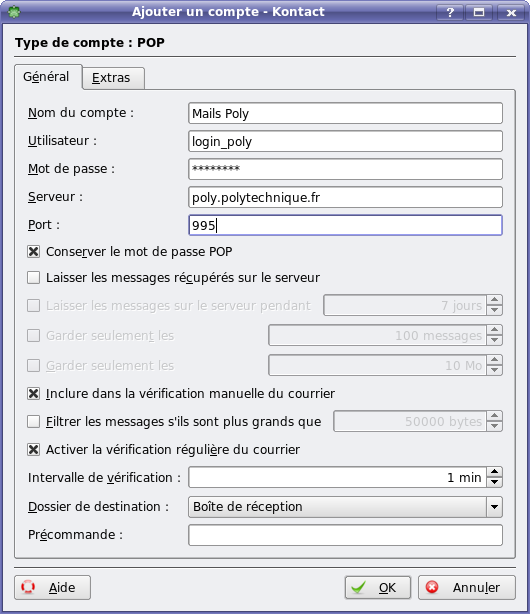
\includegraphics[width=0.48\textwidth]{images/nux_config_kmail_pop} }
      \hspace{\stretch{1}}
      \subfloat[Envoi des messages]{ 
 		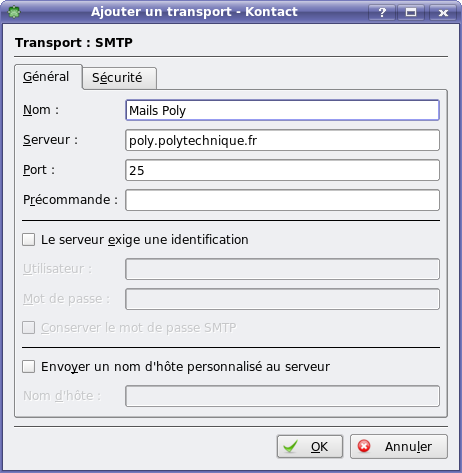
\includegraphics[width=0.48 \textwidth]{images/nux_config_kmail_smtp} }
         	 \caption{Configuration sous \app{Kmail}}
    \end{center}
  \end{figure*}


Utilise les param\`etres suivants pour configurer l'onglet \menu{G\'en\'eral} :
\begin{description}
  \item[Nom] le nom du compte, par exemple : Mails Poly
  \item[Utilisateur] rentre le \emph{login} \server{poly} que t'a fourni la DSI \`a  ton arriv\'ee sur le plateau
  \item[Mot de passe] et l\`a  le mot de passe \server{poly}
  \item[Serveur] \server{poly.polytechnique.fr}
  \item[Port] 995
\end{description}
Ensuite, va dans l'onglet \menu{Extras} et coche la case
\menu{Utiliser SSL pour s\'ecuriser les t\'el\'echargements}.

Maintenant, dans l'onglet \menu{Envoi des messages} clique sur le
bouton \menu{Ajouter\ldots}. Utilise les param\`etres suivants pour le
configurer :
\begin{description}
  \item[Nom] le m\^eme nom de compte que pr\'ec\'edemment
  \item[Serveur] \server{poly.polytechnique.fr}
  \item[Port] 25
\end{description}
Sinon, laisse toutes les cases d\'ecoch\'ees.

Tu peux aussi configurer l'acc\`es \`a  \app{l'annuaire LDAP} de l'\'Ecole, sorte de carnet d'adresses en ligne qui contient les adresses \emph{mail} de tout le monde sur le campus. Pour ce faire, commence par ouvrir \menu{Outils}, \menu{Carnet d'adresses}, puis va dans \menu{Configuration}, \menu{Configurer kAdressBook}, \menu{Consultation LDAP}. Clique ensuite sur \menu{Ajouter un h\^ote}, et configure comme suit: \\
\smallskip
\begin{minipage}[t]{0.48\textwidth}
\begin{description}
  \item[H\^ote] \server{ldap.eleves.polytechnique.fr}
  \item[Port] 389
  \item[Version de LDAP] 3
\end{description}  
\end{minipage} 
\begin{minipage}[t]{0.48\textwidth}
\begin{description}  
  \item[DN] \server{dc=polytechnique, dc=ldap, dc=eleves, dc=fr}
  \item[S\'ecurit\'e] Non
  \item[Identification] Anonyme
\end{description}
\end{minipage} \\
Une fois revenu dans \menu{Configuration LDAP}, coche la case \server{ldap.eleves.polytechnique.fr}. Tu as maintenant acc\`es \`a  l'annuaire LDAP lors de la
r\'edaction de messages, avec tout au plus un red\'emarrage de \app{Kmail}. 
%
%\imagepos{images/nux_config_ldap}{0.55}{Configuration de l'annuaire LDAP sous Kmail}{pht}
%\imagepos{images/nux_config_knode}{0.45}{Configuration de Knode}{ht}
%
\noindent
  \begin{figure*}[!h]
    \begin{center}  
      \subfloat[Configuration de l'annuaire LDAP sous Kmail]{ 
      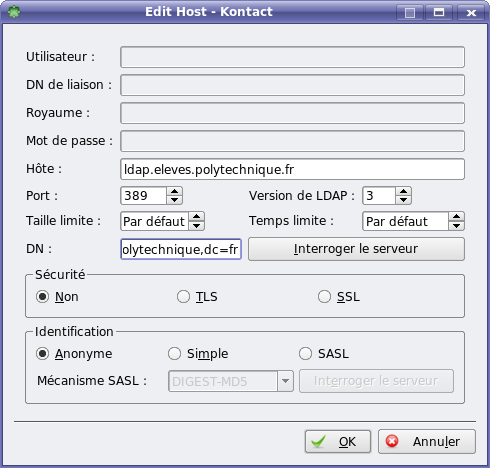
\includegraphics[width=0.48\textwidth]{images/nux_config_ldap}}
      \hspace{\stretch{1}}
      \subfloat[Configuration de Knode]{ 
 		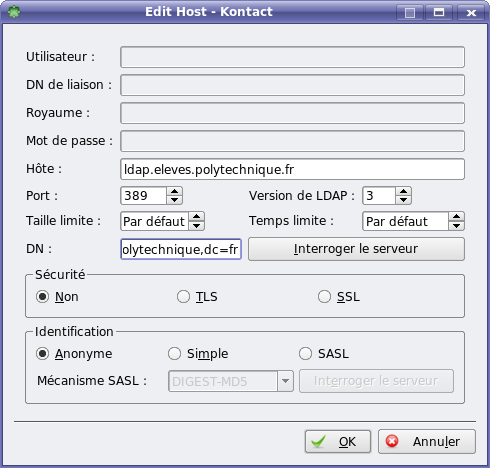
\includegraphics[width=0.48 \textwidth]{images/nux_config_ldap} }
	\caption{Configurations LDAP et \emph{news}}
    \end{center}
 \end{figure*}



%\subsubsection{Configuration \emph{news}}
%
%\flimage{images/nux_knode_icon}{0.12}{l} Le client \emph{news} le plus utilis\'e est \app{Knode}. Parmi les autres clients \emph{news}, citons 
%\app{Thunderbird}, \app{Pan} ou \app{slrn}. Ici aussi, la configuration est presque ind\'ependante du logiciel choisi.
%
%
%Sous \app{Knode}, c'est dans le menu \menu{Configuration}, puis \menu{Configurer Knode}. Va dans la rubrique \menu{Comptes, Forums de discussion} et
%cr\'ee un compte en cliquant sur \menu{Ajouter\ldots}.
%
%\imagepos{images/nux_config_knode}{0.45}{Configuration de Knode}{ht}
%
%\pagebreak
%
%Remplis l'onglet \menu{Serveur} avec les informations suivantes :
%\begin{description}
%  \item[Nom] ce que tu veux pour d\'ecrire ce compte, par exemple 'News Frankiz'
%  \item[Serveur] \server{news}
%\nopagebreak  \item[Port] 119
%\end{description}
%
%\pagebreak
% 
%Ensuite occupe-toi de l'onglet \menu{Identit\'e} :
%\begin{description}
%  \item[Nom] mets ton pseudo dans ce champ
%  \item[Organisation] X, \'Ecole polytechnique, comme tu le sens
%  \item[Adresse \'electronique] ton adresse \emph{mail}, pour que les gens puissent te r\'epondre par \emph{mail}.
%\end{description}
%
%Enfin, pour que \app{Knode} puisse envoyer des \emph{mails}, il faut aller
%dans la rubrique \menu{Comptes}, sous-rubrique \menu{Serveur de
%courrier (SMTP)}, et choisir comme serveur d'envoi de \emph{mails}
%\server{poly.polytechnique.fr}, port 25 --- c'est exactement la m\^eme
%configuration SMTP que \app{Kmail}.
%
%Si tu veux mettre une signature \`a  la fin des messages que tu
%posteras, il te suffit de la mettre dans l'onglet \menu{Identit\'e}.
%Sur la plupart des clients la signature est interpr\'et\'ee comme
%ext\'erieure au message et n'est en particulier pas incluse dans le
%texte cit\'e lorsque tu r\'eponds \`a  un message. Pour d\'efinir une
%signature \`a  la main, il suffit de mettre \verb*+-- +\ (c'est \`a  dire
%-{}-<espace>) sur une ligne, et tout ce qui suivra cette ligne
%composera ta signature.
%
%Il ne te reste plus qu'\`a  t'inscrire \`a  des \emph{newsgroups} (reporte-toi \`a  la page \pageref{newsgroups} pour plus d'infos) et \`a  poster ! \\
%
%Pour te connecter aux serveurs de \emph{news} de Polytechnique.org, qui ont un acc\`es s\'ecuris\'e, avec \app{Knode}, il y a une petite subtilit\'e car il
%ne g\`ere pas le SSL. Il faut installer \app{stunnel} qui permet de d\'efinir une redirection SSL de port. Dans \file{/etc/stunnel.conf} (ou parfois \file{/etc/stunnel/stunnel.conf}), mets les lignes suivantes (les trois premi\`eres y sont en principe d\'ej\`a ) :
%\cmdline{\# location of pid file\\
%pid = /etc/stunnel/stunnel.pid\\
%\\
%\# user to run as\\
%setuid = stunnel\\
%setgid = stunnel\\
%\\
%\# Use it for client mode\\
%client = yes\\
%\\
%\# sample service-level configuration\\
%{[}nntps{]}\\
%accept  = 1119\\
%connect = ssl.polytechnique.org:563\\
%TIMEOUTclose = 0
%}
%
%Il ne te reste plus qu'\`a  lancer \app{stunnel} par :
%\cmdline{/etc/init.d/stunnel start}
%
%Et tu peux ainsi lire les \emph{news} de Polytechnique.org en mettant \server{localhost} comme serveur et
%\server{1119} comme port. Il faut aussi que tu coches \menu{Le serveur exige une identification} et
%que tu rentres ton nom d'utilisateur \`a  Polytechnique.org et ton mot de passe, que tu peux d\'efinir
%sur \urllink{https://www.polytechnique.org/Xorg/SMTPSecurise}.

\clearpage


\newpage
\markright{Configuration sous Mac OS}
\clearpage
\pagebreak

\begin{center}

\includegraphics{images/logo_Mac}
\end{center}
\subsection{Configuration sous Mac OS X}

Voici une pr\'esentation de divers logiciels utiles pour utiliser les services propos\'es sur le r\'eseau avec Mac OS X, ainsi que leur configuration. Les logiciels non int\'egr\'es \`a Mac OS X et cit\'es ici sont quasiment tous t\'el\'echargeables sur \server{frankiz} : rubrique \menu{T\'el\'echarger -> Mac -> R\'eseau}.

\subsubsection{Configuration IP}

\flimage{images/mac_prefs_icone}{0.1}{l}
\app{Pr\'ef\'erences R\'eseau}, accessible depuis l'article de menu \menu{Pr\'ef\'erences Syst\`eme} du menu Pomme, permet de configurer la connexion au r\'eseau. Par ailleurs, si au d\'emarrage un assistant te propose de configurer ton r\'eseau, refuse gentiment et utilise la proc\'edure que le BR te propose --- c'est plus simple ;-)

La gestion des configurations r\'eseau de Mac OS X permet de cr\'eer plusieurs configurations et de passer en un clic de l'une \`a l'une autre avec le sous-menu \menu{Configuration R\'eseau} du menu Pomme, ce qui est tr\`es pratique pour les machines vou\'ees \`a �tre connect\'ees \`a plusieurs r\'eseaux successivement --- les portables par exemple. On commencera donc par cr\'eer une nouvelle configuration r\'eseau dans le menu d\'eroulant \menu{Configuration}.

\imagepos{images/mac_nouvelle_config}{0.5}{Cr\'eer une nouvelle configuration r\'eseau}{!hb}

Une fois la nouvelle configuration cr\'e\'ee, il faut configurer l'interface r\'eseau Ethernet. Dans le menu d\'eroulant \menu{Afficher}, s\'electionne \menu{Ethernet int\'egr\'e}.

\imagepos{images/mac_config_ethernet}{0.5}{Configurer l'interface r\'eseau Ethernet}{!hb}

Choisis alors \menu{Configurer IPv4} : \menu{Manuellement}. Tu trouveras toutes les valeurs d'IP n\'ecessaires pour la configuration en page \pageref{calcul_ip} ou en te reportant au screenshot suivant. Si une partie d'IP est blanche sur le screenshot, c'est qu'elle t'est personnelle et que tu dois la calculer !

\imagepos{images/mac_config_ip}{0.66}{Configuration IP}{!h}

Pour avoir acc\`es \`a Internet, il faut aussi configurer le proxy. Clique sur l'onglet \menu{Proxies}. MacOS X 10.3.3 peut utiliser un script automatique pour param\'etrer les proxies, il n'est donc pas utile de donner explicitement tous les proxies comme c'\'etait le cas avec MacOS X 10.2 et 10.3.0 ; sinon il faut mettre \server{kuzh.polytechnique.fr}, port \server{8080}. Si tu as Mac OS X 10.3.0, mets le proxy HTTP manuellement, fais toutes les mises \`a jour (Menu Pomme, \menu{Mise \`a jour de logiciels\ldots}) et ensuite tu auras l'option \menu{Configuration automatique de proxy}.

\image{images/mac_config_proxy}{0.7}{Configurer le proxy}


\subsubsection{Configuration antivirus}

Tu es sous Mac :-�

\subsubsection{Configuration web}

\flimage{images/mac_safari_icone}{0.1}{l}
\app{Safari}, le navigateur web d'Apple est maintenant enti\`erement op\'erationnel.
Un conseil : pense \`a activer le blocage des fen�tres pop-up (dans le menu \menu{Safari}). Tu peux aussi utiliser \app{Firefox} si tu pr\'ef\`eres !

\subsubsection{Configuration mail}

\flimage{images/mac_mail_icone}{0.1}{l}
\app{Mail} : un client mail, offrant les fonctionnalit\'es classiques d'un bon client : filtre antispam, r\`egles de tri automatique des mails, regroupement des mails correspondant \`a une m�me discussion.

Au premier lancement, \app{Mail} te demandera de remplir les informations concernant ton compte mail sur \server{poly}, il suffit de le remplir avec les donn\'ees suivantes :

\begin{description}
  \item[Nom complet] ton nom ! 
  \item[Adresse \'electronique] de la forme \mail{prenom.nom@polytechnique.edu}
  \item[Serveur de r\'eception] \server{poly.polytechnique.fr}
  \item[Type de compte] \menu{POP}
  \item[Nom d'utilisateur] ton login \server{poly} (les huit premi\`eres lettres de ton nom en g\'en\'eral)
  \item[Mot de passe] ton mot de passe \server{poly}
  \item[Serveur d'envoi (SMTP)] \server{poly.polytechnique.fr}
\end{description}

Si tu as d\'ej\`a cr\'e\'e un compte pr\'ec\'edemment, il faut aller dans les \menu{Pr\'ef\'erences}, onglet \menu{Comptes} (accessible depuis le menu \menu{Mail}), cr\'eer un autre compte en cliquant sur la case \menu{+} et le remplir de la m�me mani\`ere.

N'oublie pas de cocher \menu{Activer le cryptage SSL} dans l'onglet \menu{Avanc\'e}, port 995.

Cette configuration marche pour acc\'eder \`a ses mails depuis l'int\'erieur de l'X mais aussi de l'ext\'erieur, sans rien changer. Par contre depuis l'ext\'erieur tu ne peux pas envoyer de mails, car le serveur \server{poly} ne le permet pas.

\subsubsection{Configuration news}

\flimage{images/mac_thunderbird_icone}{0.1}{l}
\app{Thunderbird} : un client news permettant d'acc\'eder aux forums de discussion des \'el\`eves sur \server{frankiz} (mais aussi \`a ceux de \server{usenet} gr�ce au serveur \server{polynews.polytechnique.fr}). Il tr\`es proche d'\app{Outlook Express} dans son esprit. Dans la m�me cat\'egorie, il existe \app{MacSOUP}, \app{Unison} ou encore \app{MT-NewsWatcher}. La configuration se fait de la m�me mani\`ere.

Au premier lancement, l'application te propose d'importer les param\`etres depuis une autre application. Clique sur \menu{Suivant >}. Tu peux alors choisir quel type de compte tu veux configurer (tu remarqueras que tu peux aussi cr\'eer un compte courrier \'electronique). S\'electionne \menu{Compte forums de discussion} et clique sur \menu{Suivant >}. On te demandera alors dans l'ordre les informations suivantes :

\begin{description}
  \item[Votre nom] ton nom ou ton pseudo 
  \item[Adresse de courrier] \mail{prenom.nom@polytechnique.edu}
  \item[Serveur de forums] \server{frankiz}
  \item[Nom du compte] News Frankiz
  \item[Nom d'utilisateur] ton login poly (les huit premi\`eres lettres de ton nom en g\'en\'eral)
  \item[Serveur d'envoi (SMTP)] \server{poly.polytechnique.fr}
\end{description}

Pour t'abonner \`a des groupes de discussion, il te suffit de s\'electionner le compte \menu{News Frankiz} dans la fen�tre \menu{Dossiers} de \app{Thunderbird}, puis de cliquer sur \menu{G\'erer les abonnements aux groupes de discussion}. Tu pourras ensuite s\'electionner les forums qui t'int\'eressent parmi la liste propos\'ee. Reporte-toi \`a la page \pageref{newsgroups} pour plus d'infos sur les newsgroups auxquels t'abonner !

\subsubsection{Client FTP}
 
\flimage{images/mac_cyberduck_icone}{0.1}{l}
\app{Cyberduck} : un client FTP tr\`es simple \`a utiliser mais performant. Il te permettra d'aller t\'el\'echarger des fichiers sur les serveurs FTP des autres \'el\`eves. Il existe aussi \app{Fugu}, que certains pr\'ef\`erent.

Pour se connecter \`a un serveur, il suffit de taper son nom (exemple : \url{ftp://jtx}) dans le cadre \menu{Connexion rapide} et appuyer sur Entr\'ee.

Tu pourras ensuite naviguer sur le serveur et t\'el\'echarger ou transf\'erer des fichiers. Attention, certains serveurs configur\'es sp\'ecialement ne permettent qu'une connexion \`a la fois. Or, le t\'el\'echargement d'un fichier demande l'ouverture d'une nouvelle connexion. Il faut donc se d\'econnecter (bouton \menu{D\'econnecter}) puis lancer le t\'el\'echargement en double-cliquant sur le fichier.

Les signets te permettent de sauvegarder les serveurs sur lesquels tu te connectes souvent. Enfin, tu peux \'editer des fichiers textes directement en FTP si tu as aussi \app{SubEthaEdit}, ce qui est tr\`es commode pour modifier un site web.


\subsubsection{Autres logiciels utiles}

Voici plusieurs logiciels que tu voudras s\^urement t\'el\'echarger pour profiter au maximum des possibilit\'es du r\'eseau.\\



\flimage{images/mac_qrezix_icone}{0.1}{l}

\noindent\app{qRezix} : En deux mots, c'est un programme d\'evelopp\'e par le BR pour faciliter la vie sur le r\'eseau. Tu peux le r\'ecup\'erer dans la partie Mac de \xshare.

\noindent Pour plus de d\'etails, voir le paragraphe consacr\'e \`a qRezix \`a la page \pageref{qrezix}.

\noindent Attention, si ton firewall est activ\'e, tu dois ouvrir les ports 5050, 5053 et 5055 en TCP. Pour cela va dans \app{Pr\'ef\'erences Syst\`eme}, page \menu{S\'ecurit\'e}, onglet \menu{Coupe-feu}. S'il est \'ecrit \menu{Coupe-feu activ\'e}, clique le bouton \menu{Nouveau} et remplis la bo�te de dialogue comme sur le screenshot ci-dessous pour ouvrir les ports.\\ \\

\imagepos{images/mac_firewall}{0.5}{Ouvrir les ports pour \app{qRezix}}{!h}

\flimage{images/mac_cocoaxnet_icone}{0.1}{l}
\noindent\app{CocoaXNet} est un \'equivalent de qRezix mieux int\'egr\'e \`a Mac OS X, car il est d\'evelopp\'e en Cocoa, un langage sp\'ecifique \`a Mac OS X. \`A toi de voir !\\ \\

\flimage{images/mac_conversation_icone}{0.1}{l}
\noindent\app{Colloquy}, un client IRC dans le m�me esprit qu'\app{iChat}. Il dispose d'une interface tr\`es simple ne n\'ecessitant pas de conna�tre les commandes IRC. Tu peux te reporter \`a la page \pageref{irc} pour plus d'infos sur l'IRC. Comme autres clients IRC, on peut citer \app{Conversation}, assez proche de \app{Colloquy}, et \app{Irssix}.

\vfill

% -------------------- Puis... --------------------
\newpage
\bghdr{images/fond-infobr}
\markright{Pour continuer}
%$Id: partie2.tex 110 2005-03-02 15:56:44Z myk $
\clearpage
\section{Présentation du réseau et de plusieurs services}
\label{services}


\subsection{Une source d'informations inestimable : le WikiX}
\label{WikiX}
Bien que n'étant pas à proprement parler un service du Binet Réseau, un site un peu particulier connu sous le nom de \textbf{WikiX} est hébérgé sur un des serveurs du BR.
C'est un wiki qui rassemble toutes les informations dont tu peux avoir besoin sur le plâtal.
Le plus court moyen d'y aller est de taper \urllink{wikix} dans la barre d'adresse de ton navigateur, mais il y a aussi un lien vers le WikiX sur \fkz dans le menu navigation.

La première fois que tu te connectes sur le WikiX il faut que tu t'identifies (identification \emph{via} \urllink{polytechnique.org});
ensuite ton navigateur gardera un cookie qui t'identifiera à chaque connection si tu le souhaites. \emph{Tu ne peux lire et modifier le WikiX que si tu es identifié !}

Tu es bien entendu encouragé à contribuer au WikiX pour faire profiter les autres de ton expérience, 
soit en modifiant ou en mettant à jour un article existant, soit en créant un nouvel article qui manquait au WikiX.


Tu te rendras vite compte que \emph{peu importe l'information que tu cherches, elle est sur le WikiX.}

\subsection{Polytechnique.org}
\urllink{Polytechnique.org} est une association loi 1901 compos�e d'�l�ves et d'Anciens �l�ves
 ind�pendante de l'administration de l'�cole (et donc des domaines \server{polytechnique.fr}
 et \server{polytechnique.edu}).

Le but de l'association est la mise � disposition des X d'outils
ayant un rapport avec l'Internet, entre autres :
\begin{itemize}
  \item des redirections mails nombreuses (adresses suppl�mentaires) et � vie ;
  \item un serveur de news (comme les br.*), ouvert aux Anciens et aux non-plat�liens ;
  \item une facilitation des contacts vers les Anciens et les camarades de promotion ;
  \item une lettre mensuelle, pour s'informer sur l'actualit� de la communaut� polytechnicienne ;
  \item des annonces d'�v�nements ;
  \item des services d'h�bergement pour les groupes et binets, notemment des noms de domaine (via \server{www.po\-ly\-tech\-ni\-que.net}) et des listes de diffusion (\mail{br2005@po\-ly\-tech\-ni\-que.org}, par exemple).
\end{itemize}
Si tu veux d�couvrir les autres services de l'association ou savoir
comment les utiliser, tu peux aller sur la page
\urllink{https://www.polytechnique.org/Xorg/Xorg} (accessible depuis
le lien Documentations dans le menu de \urllink{Po\-ly\-tech\-ni\-que.org}
quand tu est connect�).

Par ailleurs, les filtres antivirus et antispam appliqu�s � sur les mails sont tr�s efficaces (99\% de rep�rage correct), et polytechnique.org te conseille donc de mettre en place la redirection suivante :
\mail{prenom.nom@polytechnique.edu}
redirig�e sur \mail{prenom.nom(.promo)@po\-ly\-tech\-ni\-que.org},
elle-m�me redirig�e vers \mail{login@poly(.po\-ly\-tech\-ni\-que.fr)}.
Pour effectuer ces redirections, connecte-toi sur les pages suivantes :
\begin{itemize}
  \item pour \mail{@polytechnique.edu} : \urllink{https://www.mail.polytechnique.edu} ;
  \item pour \mail{@polytechnique.org} : \urllink{https://www.polytechnique.org} ;
  \item pour \mail{@poly} : \urllink{http://poly.polytechnique.fr}.
\end{itemize}
Cela est expliqu� plus en d�tails sur la page
\urllink{https://www.polytechnique.org/Xorg/Re\-di\-rec\-tion\-Mails}.

Ces outils sont tr�s utiles, et faciles � s'approprier, que
ce soit pour toi, pour tes binets, ou pour (dans le
futur) garder contact avec la communaut� polytechnicienne. Rejoins
les 15000 camarades d�j� inscrits !

En cas de probl�me, n'h�site pas � contacter
\mail{contact@polytechnique.org}.


\subsection{Partager tes fichiers sur le r\'eseau avec FTP}
\bghdr{images/fond-infobr}

Les \'echanges de fichiers sur le r\'eseau \'el\`eves se font souvent par FTP. Rien de plus simple que de partager toi aussi tes pr\'ecieuses donn\'ees en installant un serveur FTP !

\paragraph{Client FTP}
Pour une utilisation basique, taper \urllink{ftp://nom-du-ftp}  (par exemple \urllink{ftp://jtx} dans la barre d'adresse de ton navigateur suffit \`a parcourir les fichiers propos\'es par \og Gentil Vieux-Chouffe \fg.
Pour une meilleure utilisation, le BR te conseille \app{FileZilla}. T\'el\'echarge-le sur \urllink{http://www.filezilla.fr} et double-clique sur l'installeur.
Tu pourras d\`es la fin de l'installation aller sur tous les FTP du r\'eseau facilement et rapidement.\\
\flimage{images/mac_cyberduck_icone}{0.07}{l} \app{Cyberduck} est un autre client FTP tr\`es simple \`a  utiliser mais performant. Il te permettra d'aller t\'el\'echarger des fichiers sur les serveurs FTP des autres \'el\`eves sans probl\`eme.\\
Pour se connecter \`a  un serveur, il suffit de taper son nom (exemple : \urllink{jtx}) dans le cadre \menu{Connexion rapide} puis d'appuyer sur Entr\'ee.\\


\paragraph{Serveur FTP}
Tu verras rapidement que tout le monde \`a  l'X poss\`ede un serveur FTP
afin de partager les diff\'erents projets, les films du JTX, ses
photos, etc. Il est donc quasiment indispensable que tu en installes un.\\

Parmi les plus simples on trouve \app{FileZilla Server} et \app{GuildFTP}, qui sont libres de surcro\^{i}t.
Si tu es sous mac, tu peux aussi jeter un \oe{}il à \app{PureFTPd Manager}, qui est très pratique à utiliser.\\
Quoiqu'il en soit, tu trouveras toutes les informations n\'ecessaires \`a la configuration de ton serveur FTP sur \urllink{http://wikix.polytechnique.org/FTP}.\\
Pense \`a lui donner un nom sur \urllink{http://dnsapp/} (voir aussi page \pageref{dnsapp})


\subsection{Avoir un nom sur le r\'eseau}


\subsection{Services propos\'es aux binets}

Le BR propose plusieurs services aux binets :
\begin{itemize}
\item une adresse \emph{mail} en \mail{nom\_du\_binet@binets.polytechnique.fr} qui permet de contacter les administrateurs \fkz\ du binet ;
\item le référencement des membres grâce au TOL ;
\item des annonces (une seule visible par binet) sur \fkz\ quand le binet veut faire de la pub ;
\item les Platalpads de binet (\urllink{http://nom\_du\_binet.platalpad}), accessibles aux membres du groupe \fkz\ (voir p. \pageref{platalpad}).
On s'y connecte en utilisant ses identifiants \fkz. Ce service fonctionne aussi \`a l'ext\'erieur via
\urllink{https://www.polytechnique.fr/eleves/platalpad/nom\_du\_binet}.
\end{itemize}

Pour disposer de ces services, il te suffit de remplir les fiches qui sont dans la case du BR à la Kès. Il faut à la création et à la passation du binet
donner au BR les noms du prez et du webmestre de ton binet ainsi que, si tu désires que ton site soit accessible à l'extérieur, une fiche pour la DSI et nous.

Le BR propose également aux binets qui le souhaite d'héberger leur site Internet. Ce site peut être interne (visible uniquement depuis l'X) ou externe (visible de l'extérieur de l'X).
Les sites binets disposent de PHP et MySQL, et bénéficient d'une capacité de stockage (extensible) de 100 Mo.

Les sites ayant une visibilité extérieure doivent satisfaire aux conditions suivantes :
\begin{itemize}
    \item Aucune information ne doit être diffusée qui pourrait nuire à l'image de l’École. (photos, vidéos, etc.) En particulier son contenu doit respecter la loi française sur les droits d'auteur.
    \item Le site doit avoir une qualité visuelle, si ce n'est professionnelle, du moins très correcte.
    \item Le site ne doit pas héberger de vidéos ou diffuser un flux vidéo (streaming). Toutes les vidéos du sites doivent être hébergées à l'extérieur. (Dalymotion, YouTube, etc.)
    \item Les images présentes sur le site ne doivent avoir une résolution suffisamment faible afin de ne pas saturer la bande passante vers l'extérieur. 
\end{itemize}

Le BR offre ce service gratuitement, en partie grâce à une subvention de la Kès.
Il se réserve le droit de refuser ou d'interrompre l'hébergement d'un site, sans préavis, sans recours possible et sans avoir à fournir de motif.
Il s'engage à en informer immédiatement le bureau du binet concerné. 

\subsection{Un outil de travail collaboratif : Platalpad}
\label{platalpad}

Platalpad est un éditeur de texte collaboratif par navigateur, un peu comme un google doc. Il permet de travailler à plusieurs sur un même document, chacun voyant les modification des autres. Il est donc très pratique pour s'organiser.\\
Il se décline en deux versions :
\begin{itemize}

\item \textbf{Platalpad généraliste :} rends-toi tout simplement sur \urllink{http://platalpad/} pour créer un nouveau document. Ensuite, il suffit de diffuser son adresse à toutes les personnes que tu veux voir prendre part à sa réalisation. \\

\item \textbf{Platalpad privé :} Chaque binet se voit automatiquement, une fois inscrit sur \fkz, attribué un espace privé, accessible seulement à ses membres. Tu peux y accéder à partir de la page \fkz du binet en question ou directement sur \urllink{http://nom-du-binet.platalpad/}. Une fois identifié, tu peux voir chacun des documents en cours de réalisation au sein du binet et les modifier à ta guise.

On s'y connecte en utilisant ses identifiants \fkz. Ce service fonctionne aussi à l'extérieur via : 
\urllink{https://www.polytechnique.fr/eleves/platalpad/nom\_du\_binet} ;

\end{itemize}

\imagepos{images/platalpad}{0.7}{Un document en cours d'édition sur un platalpad privé}{!h}

%$Id: irc.tex 144 2005-03-25 01:11:37Z myk $

\subsubsection{IRC}

\label{irc}

%IRC est un autre moyen de communication mis à ta disposition par le Binet Réseau. Il s'agit d'un système de \emph{chat} (messagerie instantanée) permettant à la fois de dialoguer à plusieurs dans des \emph{salons}, mais également d'avoir des conversations privées avec d'autres personnes connectées.

IRC is a communication device provided by the Binet Reseau. It is a \emph{chat} software
enabling a multi-user conversation within \emph{channels}, as well as private chats with other connected people.

The Binet Reseau's IRC server is connected to RezoSup, an IRC network gathering lost of french engineering schools and universities.

%Le serveur IRC du Binet Réseau est relié à RezoSup, réseau IRC des grandes écoles d'ingénieurs et université française.

%Pour te connecter sur IRC tu disposes de deux méthodes:
There are two ways for you to connect to IRC :


\begin{description}
  \item[using an IRC client:] we recommend the use of \app{X-Chat} (available in the \emph{Télécharger} part on  \fkz). Use \server{ircserver} as server, and \server{6667} (default port) as port.
  \item[using the web interface:] go to \urllink{http://ircserver/}, or follow the link \menu{Accéder à IRC} on \fkz. Thus you'll be able to use the IRC without installing anything.
 \end{description}

Here are some channels you might find usefull :
 \begin{itemize}

  \item \ngname{\#x} the channel for all students at the Ecole Polytechnique.
  \item \ngname{\#linux} if ever you have questions about linux
  \item \ngname{\#superquizz} an online quizz(type \texttt{!nick x} when login in)
  \item \ngname{\#br} the Binet Reseau's channel
 \end{itemize}


%
\subsubsection{Le site du BR : un Wiki}
\label{siteBR}

Le site public du Binet R�seau est disponible sur \url{http://frankiz/binets/reseau/}. C'est un wiki, ce qui permet aux BR-men de le mettre ais�ment
� jour avec les derni�res informations de configuration.

Tu y trouveras un grand nombre d'informations � jour sur le BR, sur les services que nous offrons, et sur nos projets.

Il est compl�mentaire � la {\sc FAQ} et � cet InfoBR : il contient
des informations de configuration pour les services offerts par le
BR et des d�tails pour les projets que le BR m�ne.


%%$Id: qrezix.tex 144 2005-03-25 01:11:37Z myk $

\subsection{La t\'el\'evision du BR}
\label{TV}

Le BR diffuse sur le r\'eseau plusieurs dizaines de chaines de t\'el\'evision et radios. Pour les recevoir, nous recommandons \app{vlc}, disponible sur le X-Share.

\subsubsection{Configuration de vlc}

La liste des cha\^ines est diffus\'ee sous forme d'annonces SAP. Pour voir ces annonces, ouvre ta liste de lecture (Vue -> Liste de lecture), et active la d\'ecouverte de services (\ref{vlc:config}).
Attention sous \app{Windows Vista} un probl\`eme de compatibilit\'e connu entra\^ine un \'ecran noir. Pour le r\'esoudre le BR t'a pr\'epar\'e une page sur le Wikix.

\imagepos{images/vlc_config_sap.png}{0.75}{Configuration de vlc pour la t\'el\'evision par le r\'eseau}{h!}\label{vlc:config}

Tu auras ainsi dans ta liste de lecture les diff\'erents cha\^{i}nes disponibles.

\subsubsection{Autre m\'ethode}

Si ton client pr\'ef\'er\'e ne supporte pas les annonces SAP, ou que les annonces SAP ne marchent pas chez toi, tu peux r\'ecup\'erer la liste des cha\^ines par
PodCast, à l'adresse \url{http://tv.eleves.polytechnique.fr/tvbr.xml}. Sous \app{vlc}, active la d\'ecouverte des services PodCast dans la liste de
lecture (G\'erer > D\'ecouverte de services > Podcast), puis va dans Param\`etres > Pr\'ef\'erences > Liste de Lecture > D\'ecouverte de services > Podcast et
met l'adresse \url{http://tv.eleves.polytechnique.fr/tvbr.xml} dans le champ \guillemotleft~Liste des URLs~\guillemotright .

\subsubsection{Et si ça ne marche toujours pas?}

V\'erifie que tu utilises bien la derni\`ere version de \app{vlc}. Les versions inf\'erieures à 0.8.5 sont connues pour ne pas fonctionner.

Si rien ne marche, la raison la plus probable est un \emph{firewall} qui intercepte les flux t\'el\'es. Configure ton \emph{firewall} afin d'autoriser
ces flux. Sous Linux, les r\`egles \emph{iptables} suivantes suffisent:

  \cmdline[0.85] {
   -A INPUT -i eth0 -d 224.0.0.0/24 -j ACCEPT
   -A INPUT -i eth0 -d 239.255.42.0/24 -s 192.168.225.0/24 -p udp -m udp --dport 1234 -j ACCEPT
   -A INPUT -i eth0 -d 239.255.255.255/32 -p udp -m udp --dport 9875 -j ACCEPT
   -A OUTPUT -o eth0 -d 224.0.0.0/4 -j ACCEPT.
  }


\subsection{Installer et mettre à jour Windows ou Linux}

\subsubsection{Licences de produits Microsoft}
\label{msdnaa} Les accords n\'egoci\'es par le BR avec Microsoft dans le cadre de MSDNAA donnent \`a  chaque X le droit de poss\'eder une version de Windows
XP Pro, de Windows Vista Business ou de Windows 7 Pro gratuite et l\'egale, ainsi que les licences pour la plupart des logiciels de la soci\'et\'e (quasiment tous, sauf
Office et les jeux). La seule condition \`a  remplir est d'\^etre \'etudiant sur le pl\^atal au moment de l'installation du logiciel ; tu pourras ensuite le
garder sur ton PC m\^eme apr\`es ton d\'epart de l'X.

La proc\'edure pour obtenir les logiciels et les cl\'es correspondantes
est la suivante :
\begin{itemize}

\item Va d'abord sur \fkz et connecte-toi, puis clique sur le lien \menu{Licences MSDNAA} qui se trouve dans la rubrique \menu{Administration}. S\'electionne le logiciel que tu souhaites installer et valide ta demande, tu recevras ta cl\'e par e-mail. Facile ! Si jamais le logiciel n'est pas dans la liste propos\'ee, c'est soit qu'il n'y a pas besoin de cl\'e --- c'est le cas de beaucoup des logiciels autres que Windows, soit qu'on a oubli\'e de l'y mettre ; dans ce cas, \'ecris \`a  \mail{msdnaa@eleves} pour qu'on t'attribue manuellement une cl\'e.

\item Maintenant que tu as ta cl\'e, il faut t\'el\'echarger le logiciel proprement
dit. Pour cela, connecte-toi par FTP sur \urllink{ftp://miroir/windows/msdnaa/} avec ton client FTP pr\'ef\'er\'e. Tu pourras, selon le logiciel, y r\'ecup\'erer soit une image du CD de type \file{logiciel.iso} (\`a 
graver ou \`a  utiliser avec \app{Daemon Tools}), soit directement le contenu du CD.
 
\end{itemize}

\subsubsection{Miroirs GNU/Linux}

Le BR propose sur \urllink{ftp://miroir/} des miroirs de plusieurs distributions GNU/Linux. Leur avantage principal est que le téléchargement se fait directement sur le réseau local, donc \emph{très} rapidement.
Les miroirs suivants sont disponibles:

\begin{itemize}
\item \distrib{Cygwin} (Environnement Unix pour Windows);
\item \distrib{Debian} (CDs, distribution et mises à jour);
\item \distrib{Gentoo} (CDs, distribution et mises à jour);
\item \distrib{Ubuntu} (CDs, distribution et mises à jour);
\item \distrib{Fink} (Nombreux logiciels Unix/Linux adaptés pour Mac OS).
\end{itemize}

Les miroirs évoluent régulièrement. Tu peux te référer \`a la page \pageref{ubuntu_mirror} pour leur configuration sous \distrib{Ubuntu} ;
pour les autres, toutes les informations pour leur utilisation sont disponibles sur \urllink{https://br.binets.fr/Miroir\_FTP}.

%Pour Windows, les fichiers ISO \`a  t\'el\'echarger sont les suivants :
%\begin{description}
%\item[Pour Windows XP]
%\urllink{ftp://miroir/windows/msdnaa/Windows\%20XP/Francais/fr\_windows\_xp\_professional\_with\_service\_pack\_3\_x86\_cd\_x14-80440.iso}.
%
%\item[Pour Windows Vista]
%L\`a , il y a deux possibilit\'es :
%\begin{description}
%\item[Si tu as un processeur 64 bits :] L'image \`a  t\'el\'echarger est dans\\
%\urllink{ftp://miroir/msdnaa/win\_vista\_business\_avec\_sp1/dvd\_64bits/francais/}. Attention, cette
%image ISO est \`a  graver sur un DVD. On remarque aussi que parfois, m\^eme sur un processeur 64 bits il
%vaut mieux choisir la version 32 bits de Windows (celle qui est dans le prochain \emph{item}) pour des
%raisons de disponibilit\'e de pilotes.
%\item[Si tu as un processeur 32 bits :] L\`a , tu peux choisir de graver :
%\begin{itemize}
%\item soit un DVD, dans \\
%\urllink{ftp://miroir/msdnaa/win\_vista\_business\_avec\_sp1/dvd\_32bits/francais/};
%\item soit quatre CDs, que tu trouveras dans \\
%\urllink{ftp://miroir/msdnaa/win\_vista (version CD)/cd\_32bits/french/}.
%
%\end{itemize}
%\end{description}
%
%\item[Pour Windows 7]
%Comme pour Vista, deux possibilit\'es selon ton processeur. Attention, les images sont \`a graver sur DVD :
%\begin{description}
%\item[Si tu as un processeur 64 bits :] L'image \`a  t\'el\'echarger est dans\\
%\urllink{ftp://miroir/msdnaa/win\_7/french/64 bits/}.
%\item[Si tu as un processeur 32 bits :] L'image \`a  t\'el\'echarger est dans\\
%\urllink{ftp://miroir/msdnaa/win\_7/french/32 bits/}.
%
%\end{description}
%\end{description}
%
%Les versions anglophones de Windows XP, Vista et 7 sont \'egalement disponibles sur \server{miroir}.
%Ainsi, si tu as achet\'e un ordinateur sans OS (et ainsi \'economis\'e environ 150 \euro), tu vas chez un copain, fais les demandes et graves le CD chez lui. Si tu as encore des questions, plus de d\'etails sont donn\'es dans le Wikix et le WikiBR de \fkz.
%



%\subsection{Descriptions des différents serveurs}
{\bf Serveurs du BR :} Voici la liste des serveurs du BR que tu vas
utiliser le plus durant tes deux années sur le platâl, ainsi que
leurs adresses IP et les services qu'ils hébergent. Note que ces services
peuvent à tout moment migrer d'une machine à une autre en cas de
besoin.


\begin{description}
        \item[frankiz] (\server{129.104.201.51}) : DNS secondaire,
        \emph{news}, portail des élèves, sites des binets
        \item[gwennoz] (\server{129.104.201.52}) : DNS secondaire,
        développement, miroirs FTP
        \item[heol] (\server{129.104.201.53}) : DNS principale,
        serveur \app{xNet} (pour \app{qRezix}, voir page~\pageref{qrezix}), serveur IRC
        \item[skinwel] (\server{129.104.201.54}) : DNS secondaire,
        dépôt SVN, télévision
	\item[pellwel] (\server{129.104.201.57}) : télévision
    \item[enez] (\server{129.104.201.61}) : Domaine windows, MSDNAA (logiciels Microsoft gratuits)
\end {description}

{\bf Serveurs de la DSI : } \'Etant donné que le réseau élèves est un
sous-réseau de celui de la DSI, nous utilisons également les
serveurs de celle-ci et les services qu'ils hébergent.

\begin{description}
        \item[kuzh] (\server{129.104.247.2}) : \emph{proxy} http (pour l'Internet), \emph{proxy} ssh pour sortir du plateau, futur \emph{proxy} ftp
        %\item[sil] (\server{129.104.247.3}) : ancien \emph{proxy} ssh double sens et \emph{proxy} ftp en sursis, il est conservé tant qu'il survit, et ne sera pas réparé s'il a des problèmes.
        \item[poly] (\server{129.104.247.5}) : \emph{mails} (réception, envoi), tu trouveras en t'y connectant en http (\urllink{http://poly/}) le certificat de sécurité pour l'authentification sécurisée.
        \item[moned] : serveur d'authentification, permettant de
        changer ton mot de passe \server{moned}. Ce mot de passe est celui qui
        te permet de te connecter et d'utiliser n'importe
        quelle machine de salle info. Ton travail n'étant pas stocké
        en local, il t'est donc accessible quel que soit le PC des salles info depuis
        lequel tu te connectes.
    \item[milou] : serveur NTP (\server{ntp.polytechnique.fr})
\end {description}

\fbox{
\begin{minipage}{0.9\textwidth}
  \bf ATTENTION : Les serveurs de la DSI sont à ta disposition pour
  des usages bien précis et ne servent pas de serveurs de
  stockage. La DSI est assez vigilante
  et elle a pour habitude de sanctionner les abus; cela peut inclure la perte de tes comptes
  \server{poly}, \server{moned} ou \server{sil}.
\end{minipage}
}


\newpage


% -------------------- Enfin -------------------
%$Id: partie2.tex 110 2005-03-02 15:56:44Z myk $

\section{R�f�rence Rapide}

\subsection{Polytechnique.org}
\url{Polytechnique.org} est une association loi 1901 compos�e
d'�l�ves et d'anciens �l�ves
 ind�pendante de l'administration de l'�cole (et donc des domaines \server{polytechnique.fr}
 et \server{polytechnique.edu}).

Le but de l'association est la mise � disposition des X d'outils
ayant un rapport avec l'Internet. En particulier, parmi ces outils
il y a :
\begin{itemize}
  \item des redirections mails nombreuses (adresses suppl�mentaires) et � vie ;
  \item des services de news comme le binet r�seau, mais ouverts aux anciens, et aux non plat�liens ;
  \item des contacts ais�s vers les anciens, les camarades de promotion ;
  \item une lettre mensuelle, pour publier des informations qui toucheront tous les polytechniciens ;
  \item des annonces d'�v�nements ;
  \item des services d'h�bergement pour les groupes et binets, des noms de domaine (via \server{www.po\-ly\-tech\-ni\-que.net}) ;
  \item des listes de diffusion de mails (\mail{br2005@polytechnique.org}, par exemple).
\end{itemize}

Par ailleurs, les filtres antivirus et antispams de polytechnique.org �tant assez efficaces, nous te conseillons de mettre en place la redirection
suivante : adresse \mail{prenom.nom@polytechnique.edu} redirig�e sur l'adresse \mail{prenom.nom(.promo)@polytechnique.org}, elle-m�me redirig�e vers
l'adresse \mail{login@poly(.polytechnique.fr)}. Pour effectuer ces redirections, connecte-toi sur les pages suivantes :
\begin{itemize}
  \item pour l'adresse \mail{@polytechnique.edu} : \url{https://www.mail.polytechnique.edu/} ;
  \item pour l'adresse \mail{@polytechnique.org} : \url{http://www.polytechnique.org} (elle est dr�le celle-l�, hein ?) ;
  \item pour l'adresse \mail{@poly} : \url{http://poly.polytechnique.fr}.
\end{itemize}

Tu remarqueras tr�s rapidement que ces outils sont tr�s utiles, que
ce soit pour toi personnellement ou pour tes binets et pour, dans le
futur, garder contact avec la communaut� polytechnicienne: rejoins
les 13000 camarades d�j� inscrits !


%$Id: questions_reponses.tex 144 2005-03-25 01:11:37Z myk $

\subsection{Questions-réponses}

Les questions les plus courantes sont répertoriées ici pour te faire gagner du temps !

\begin{description}

\item[J'ai une question sur l'informatique] je cherche sur le WikiBR et/ou demande \`a un BRman.

%\item[J'ai perdu mon mot de passe qRezix] je le re-définis dans \menu{Administration / Compte / Mes données réseau} sur \fkz ou directement sur \urllink{http://xnetserver}.

\item[Je veux voir mon pseudo quand j'ai voté à la QDJ] je définis mon pseudo sur ma fiche \linebreak trombino sur la page \menu{Administration / Compte / Profil} sur \fkz.

\item[J'ai un deuxième ordinateur, qu'est-ce que je fais ?] je demande une deuxième adresse IP en envoyant un mail à \mail{root@eleves.polytechnique.fr} en préfixant le sujet par [IP] 

\item[Je n'ai plus de réseau] je vais voir la 4\ieme de couverture.

\item[Je viens de changer de casert/section, il faudrait mettre à jour ma fiche TOL] j'envoie \linebreak un mail à \mail{tol@frankiz} avec les modifications à effectuer ainsi que la raison de ces
modifications.

\item[Mon client mail dit que \guillemotleft~l'autorité de certification est inconnue~\guillemotright ] je vais télécharger le certificat de sécurité sur \urllink{https://poly/} et je l'installe.

\item[Je ne reçois pas mes mails] je vérifie ma redirection sur \urllink{http://poly}.

\item[Si la boite mail poly est saturée] Je me connecte sur :\\
\urllink{https://webmail.enseignement.polytechnique.fr/imp/login.php}, 
login : nom de famille --
password : mdp enex ; et je supprime mes mails.


\item[Je n'arrive pas à me connecter à \server{poly}] j'essaye \server{poly.polytechnique.fr}.

\item[Mon ordinateur n'a pas de nom sur le réseau] je lui en donne un gr\^ace \`a \urllink{http://dnsapp/} .

\item[Je cherche des informations sur l'Ecole] je regarde sur \urllink{http://intranet}.

\item[Je cherche à joindre une personne de l'administration] l'annuaire de l'École est sur \linebreak{} \urllink{http://annuaire/}.

\item[Je cherche le numéro de portable d'un X] \urllink{http://www.polytechnique.org}.

\item[J'aimerais être un geek moi aussi !] j'apprends par c\oe ur \urllink{9gag.com/}.

\end{description}


\subsection{Membres \'eminents du Binet R\'eseau}

Chaque BR-man signale quels syst\`emes d'exploitation il conna\^it.

\mbr{Sigma}{71 66}{\wins \nuxs}{Prez, root, news, devel qrezix, support@windows, support@linux}{Touche à tout, il essaie de suivre tout ce qui se passe (même s'il subit parfois ce qui se passe sur les machines). Il a découvert les Virtualbox et s'amuse à les multiplier. Il se charge de la permanence BR matinale (dès 5-6 heures du matin !)}

\mbr{Nathaniel}{76 83}{\nuxs \wins}{Trez, root, web, tol, news, IRCop, devel@frankiz}{Tyran bisounours des news. Si tu as une question concernant le BR (sauf le support), appelle le, y a de grandes chances que ça le concerne. Sa vie a changé depuis qu'il a découvert la puissance du ssh (puis, plus tard, la puissance du -Y).}

\mbr{J-Philippe}{76 42}{\nuxs}{root, web, tol, news, InfoBR, support@linux, support@\LaTeX{}}{Passionné de typographie et de \LaTeX{}, il était logique que ce soit lui qui s'occupe de l'InfoBR. Ne parle surtout pas de majuscule devant lui, il te prendrait la tête pendant 2 heures pour t'expliquer la différence avec la capitale. \`A part ça, il essayera toujours de trouver un peu de temps pour t'aider si tu as un problème en linux (c'est pas le meilleur) ou en \LaTeX{} (c'est le meilleur!).}

\mbr{simon}{73 75}{\nuxs}{root, IRCop, bll}{Depuis assez peu de temps sous linux, il essaie d'en maîtriser les arcanes les plus t\'en\'ebreuses. Toujours à la rue, mais à un degr\'e variable selon l'heure et le jour.}

\mbr{Totor}{71 96}{\macs}{root, web, tol, news, support@mac, Xshare@mac}{Toujours prêt à aider les macqueux, même en plein milieu de la nuit, et les autres aussi même si il ne comprend pas leur problèmes. Tu le trouveras à coup sûr entre entre son kazert et le BôB dès la fin des cours. Pour les macs addicts, ils trouveront leur bonheur et tous les petits programmes qui vont bien sur son ftp.}

\mbr{Andrei}{76 98}{}{devel@root, devel@frankiz}{}

\mbr{Kithyane}{76 22}{\nuxs \wins}{web, tol, news, BRwoman, devel@frankiz}{Elle a découvert son côté geek en entrant au BR, est passée sous Linux depuis, et s'émerveille des nouvelles possibilités qui s'offrent à elle. Extension spirituelle de Nathaniel pour les validations sur Frankiz et la modération des br, en un peu moins bisounours, peut-être, mais avec le sourire de la BRWoman en plus !}

\mbr{Mikado}{70 90}{\wins}{admin@windows}{Problème avec Windows ou les licences Microsoft ? C'est pour lui!}

\mbr{Jiherr}{72 60}{\macs}{support@mac, respo mac, relex}{}

\mbr{RogerTroutman}{77 00}{\wins}{root, admin@windows, support@windows}{}

\mbr{Boris}{73 70}{\nuxs}{root, devel@qrezix}{Gentooiste, il a choisi la voie de la concaténation des Saints Manuels. Il a abandonné son humanité depuis peu pour devenir une page de manuel à  part entière. Tapez `\texttt{/}' pour rechercher.  }

\mbr{Bruno}{71 29}{\nuxs}{support@linux}{N'hésite pas à m'appeler si tu as un problème avec Linux ou le réseau.}

\mbr{Pom}{77 12}{\wins \nuxs}{web, tol, support@windows, support@linux, support@\LaTeX{}}{Coucou ! Moi c'est Pom (ah mince c'est marqué à gauche... bon ben
sinon, c'est Thomas, ça c'est une info exclusive !). Je suis toujours
prêt à t'aider si tu as le moindre problème ou la moindre question.
Mon but c'est rendre service, donc n'hésite pas ! Ma porte est
toujours ouverte (certes elle est perdue au milieu du 3ème étage de
Maunoury, mais quand même). Je sais comment fonctionne Windows :
clic gauche sur le menu démarrer, puis encore un clic au bon
endroit, et ... Quant à linux, et bien je sais que si je tape
"firefox" j'arrive sur internet ! C'est déjà ça. Sinon je m'y connais
en latex, enfin \LaTeX{} hein! Pas de mauvaise compréhension ;) et je
suis chargé de valider tes annonces frankiz, c'est toujours bon à
savoir ! Bisous !}

\mbr{Ninja}{70 70}{\nuxs}{devel@root, BLL, support@linux}{}

\mbr{Shuba}{71 32}{\nuxs}{devel@root}{}

\mbr{fulanor}{72 56}{\macs}{news}{}

\mbr{Buu-Minh}{72 17}{\nuxs \wins}{devel@root, support@windows, support@linux}{Même si ça ne se voit pas, il sera toujours prêt à t'aider si tu rencontres un problème avec ta machine.}


\subsubsection*{Description rapide des postes}

\begin{description}

  \item[Prez]{(\mail{prez@frankiz}) Poste fictif, qui permet toutefois d'avoir
des relations bien plac\'ees.}

  \item[Trez]{(\mail{trez@frankiz}) Escroc qui cherche uniquement \`a remplir le compte en banque pour organiser un voyage de geeks \`a Redmond, ou plut\^ot Cupertino\dots}

  \item[relex]{Assistant du prez pour les relations avec les \emph{gens}.}

  \item[root]{(\mail{root@frankiz}) Les roots sont les administrateurs du r\'eseau. Ce sont eux qui s'\'evertuent \`a maintenir en \'etat de marche les serveurs, \`a rajouter de nouveaux services et \`a rep\'erer les boulets qui font de la merde sur le r\'eseau. S'il s'agit de g\'erer un compte de binet, utilise plut\^ot \mail{binets@frankiz}.}

  \item[admin@windows] {(\mail{windows@frankiz}) Administrateurs du domaine Windows. En cas de probl\`eme avec Windows, en particulier avec l'antivirus, ce sont les mieux plac\'es pour t'aider ; bien s\^ur c'est plus facile si tu es sur le domaine !
}
  \item[support@windows] {(\mail{support@frankiz}) SOS d\'epannage windows, j'\'ecoute ! Pr\^ets \`a tout pour sauver une jeune demoiselle (ou un jeune \emph{gens} \`a la rigueur) en d\'etresse avec son windows\dots }

  \item[support@mac] {(\mail{support@frankiz}) C'est un poste naturellement tranquille. Qui a besoin d'\^etre d\'epann\'e sur Mac? Ah, c'est vrai : celui qui a install\'e Windows dessus en suivant les conseils de l'InfoBR... }

  \item[devel]{Joyeux programmeurs qui sont l\`a pour am\'eliorer les logiciels du BR --- \app{qRezix} et ses plug-ins (\mail{qrezix@frankiz}), le site web \urllink{http://frankiz/}. Ce sont eux qui tous les deux mois te disent que ton \app{qRezix} n'est pas \`a jour.}

  \item[news] {(\mail{news@frankiz}) Mainteneurs du serveur de news, ils surveillent aussi ce que tu postes et que tu respectes les r\`egles de base comme les crossposts (marteau-th\'erapie) \mbox{;-)}}

  \item[web@frankiz] {(\mail{web@frankiz}) Webmestres de \fkz, ils valident les annonces et les activit\'es et surveillent le contenu du site de ton binet ou de ton site perso.}

  \item[X-share] {(\mail{xshare@frankiz}) Personne sympathique qui cherche \`a longueur de temps de nouveaux logiciels gratuits, ou mieux, libres, \`a proposer aux \'el\`eves dans \xshare.}

  \item[InfoBR]{L'art du travail distribu\'e: il dit \`a tous les autres d'\'ecrire. Le probl\`eme majeur \'etant la synchronisation des diff\'erentes parties avant les dates limites.}

  \item[TV]{Charg\'es de maintenir la diffusion de la t\'el\'e sur le r\'eseau. Changeurs de cha\^ine, dieux du multicast, ils sont les amis des switches\dots\ ou pas.}

  \item[QDJ Master] {(\mail{qdj@frankiz}) Chaque jour un nouveau dilemne sur \fkz\dots\ n'h\'esitez pas \`a faire vos propositions \`a \urllink{qdj@frankiz}.}

  \item[IRCop]{Responsable des relations avec RezoSup. Viendez sur IRC (\urllink{http://ircserver/}) !}

  \item[TOL] {(\mail{tol@frankiz}) V\'erificateur de photos, il surveille le Trombi On Line.}

  \item[BRwoman]{Preuve vivante que le BR n'est pas un milieu enti\`erement masculin.}

\end{description}


%$Id: lexique.tex 144 2005-03-25 01:11:37Z myk $

\subsection{Lexique}

\begin{description}
  \item[Avaya] Fournisseur de coupures r�seau.
  \item[BR] Binet R�seau : le binet qui s'occupe d'administrer le r�seau des �l�ves, de d�velopper et de maintenir le site \url{http://frankiz/} et le logiciel \app{qRezix}.
  \item[Client] (voir serveur) : programme qui permet de se connecter � un serveur. Par exemple un client news (comme \app{Thunderbird}), un client FTP (comme \app{SmartFTP}), un client xNet (comme \app{qRezix})
  \item[Crosspost] mot pr�f�r� des newsmestres qui entra�ne souvent une avalanche de mails d'insultes. D�crit l'art et la mani�re de ne pas pourrir les \emph{newsgroups}.
  \item[DNS] \emph{Domain Name Server} : associe un nom de machine � une IP, par exemple \server{frankiz} � 129.104.201.51.
  \item[DSI] (Direction des Syst�me d'Information) ce sont eux qui g�rent tout le mat�riel informatique de l'�cole, ton t�l�phone, ton acc�s internet, tes mails\ldots\ un conseil : ne joue pas au plus malin avec eux.
  \item[FAQ] (Foire Aux Questions, ou \emph{Frequently Asked Questions}) c'est l� que tu peux trouver des r�ponses classiques ou m�me quelques trucs et astuces
  \item[Firewall] Logiciel de protection de ton ordinateur contre les infiltrations de vers ou de pirates informatiques.
  \item[FTP] \emph{File Transfer Protocol} : protocole r�seau qui permet de s'�changer des fichiers.
%  \item[InfoBR] tu l'as entre les mains.
  \item[IP] Adresse de ton ordinateur sur le r�seau, compos�e de quatre nombres compris entre 0 et 255 ($129.104.xxx.xxx$). Elle identifie ta machine aupr�s des autres utilisateurs du r�seau.
  \item[proxy] machine qui autorise (et du m�me coup restreint) les communications avec l'ext�rieur. Le \emph{proxy} prot�ge tous les ordinateurs du r�seau des attaques.
%  \item[R�solution DNS] trouver l'IP associ�e � un nom DNS pour pouvoir se connecter � la machine concern�e.
  \item[RTF*] \emph{Read The Fucking}\ * : allusion sympathique au fait que tu aurais pu trouver l'information autre part\ldots\ tout pr�s souvent (voir RTFIBR, RTFFAQ, RTFM, etc.)
  \item[RTFFAQ] tu devrais trouver la r�ponse � ta question dans la FAQ sur \fkz.
  \item[RTFIBR] il semblerait que la r�ponse soit dans l'InfoBR. Souvent suivi du num�ro de la page. L'usage de cette expression est traditionnellement associ� au mot crosspost.
  \item[RTFM] M, c'est le manuel, le reste on l'a d�j� expliqu� ;-)
  \item[serveur] (voir client) : programme qui permet d'accueillir des services. Comme par exemple le partage de fichier, le voisinage r�seau, un site web\ldots\
  \item[Serveur] (ce n'est pas le m�me qu'avant ;-)) : machine qui accueille des serveurs (l� c'est celui d'au-dessus). Le BR poss�de des serveurs soigneusement cach�s dans une salle secr�te et blind�e.
  \item[SSH] Connexion permettant de travailler sur une machine distante.
  \item[STFW] variante : \emph{Search The Fucking Web}. \url{http://www.google.fr} est ton ami.
  \item[Troll] d�bat pol�mique sans fin permettant de d�ployer la mauvaise foi des deux parties.
%  \item[Z�bulon] �a veut rien dire, mais c'�tait juste pour avoir un mot en Z.
\end{description}


\vfill


\end{document}
